%% RiSE Latex Template - version 0.5
%%
%% RiSE's latex template for thesis and dissertations
%% http://risetemplate.sourceforge.net
%%
%% (c) 2012 Yguaratã Cerqueira Cavalcanti (yguarata@gmail.com)
%%          Vinicius Cardoso Garcia (vinicius.garcia@gmail.com)
%%
%% This document was initially based on UFPEThesis template, from Paulo Gustavo
%% S. Fonseca.
%%
%% ACKNOWLEDGEMENTS
%%
%% We would like to thanks the RiSE's researchers community, the 
%% students from Federal University of Pernambuco, and other users that have
%% been contributing to this projects with comments and patches.
%%
%% GENERAL INSTRUCTIONS
%%
%% We strongly recommend you to compile your documents using pdflatex command.
%% It is also recommend use the texlipse plugin for Eclipse to edit your documents.
%%
%% Options for \documentclass command:
%%         * Idiom
%%           pt   - Portguese (default)
%%           en   - English
%%
%%         * Text type
%%           bsc  - B.Sc. Thesis
%%           msc  - M.Sc. Thesis (default)
%%           qual - PHD qualification (not tested yet)
%%           prop - PHD proposal (not tested yet)
%%           phd  - PHD thesis
%%
%%         * Media
%%           scr  - to eletronic version (PDF) / see the users guide
%%
%%         * Pagination
%%           oneside - unique face press
%%           twoside - two faces press
%%
%%		   * Line spacing
%%           singlespacing  - the same as using \linespread{1}
%%           onehalfspacing - the same as using \linespread{1.3}
%%           doublespacing  - the same as using \linespread{1.6}
%%
%% Reference commands. Use the following commands to make references in your
%% text:
%%          \figref  -- for Figure reference
%%          \tabref  -- for Table reference
%%          \eqnref  -- for equation reference
%%          \chapref -- for chapter reference
%%          \secref  -- for section reference
%%          \appref  -- for appendix reference
%%          \axiref  -- for axiom reference
%%          \conjref -- for conjecture reference
%%          \defref  -- for definition reference
%%          \lemref  -- for lemma reference
%%          \theoref -- for theorem reference
%%          \corref  -- for corollary reference
%%          \propref -- for proprosition reference
%%          \pgref   -- for page reference
%%
%%          Example: See \chapref{chap:introduction}. It will produce 
%%                   'See Chapter 1', in case of English language.
%%
%% Citation commands:
%%          \citet (from natbib) -- To cite a reference as part of the narrative
%%          \citep (from natbib) -- To cite a reference between parenthesis
%%          citationblock environment -- To produce direct citation blocks according to the ABNT

\documentclass[pt,twoside,onehalfspacing,bsc]{risethesis}
\usepackage[brazil]{babel}
\usepackage[utf8]{inputenc}

\usepackage{colortbl}
\usepackage{color}
\usepackage[usenames,dvipsnames,svgnames,table]{xcolor}
\usepackage{microtype}
\usepackage{bibentry}
\usepackage{subfigure}
\usepackage{multirow}
\usepackage[figuresleft]{rotating}
\usepackage{booktabs}
\usepackage{pdfpages}
\usepackage[style=base]{caption}
\usepackage{lipsum}
\usepackage{sectsty}
\usepackage{listings}
\usepackage{hyphenat}
\usepackage{float}
\usepackage{multicol}
\usepackage{rotate}

% \captionsetup[table]{position=top,justification=centering,width=.85\textwidth,labelfont=bf,font=footnotesize}
% \captionsetup[lstlisting]{position=top,justification=centering,width=.85\textwidth,labelfont=bf,font=footnotesize}
\captionsetup[figure]{position=bottom,justification=centering,width=.85\textwidth,labelfont=bf,font=footnotesize}

%% Chapter and (Sub)Section fonts must be same size as text (12)
\sectionfont{\fontsize{12}{15}\selectfont}
\subsectionfont{\fontsize{12}{15}\selectfont}
\subsubsectionfont{\fontsize{12}{15}\selectfont}

%% Change the following pdf author attribute name to your name.
\usepackage[linkcolor=black,
            citecolor=black,
            urlcolor=black,
            colorlinks,
            pdfpagelabels,
            pdftitle={Monografia de Michelle Araujo},
            pdfauthor={Michelle Araujo},
            breaklinks=true]{hyperref}
            
\newcommand{\quotes}[1]{``#1''}

\address{SALVADOR}

\universitypt{Universidade Federal da Bahia}
\universityen{Federal University of Bahia}

\institutept{Instituto de Matemática e Estatística}
\instituteen{Institute of Mathematics and Statistics}

\departmentpt{Departamento de Ciência da Computação}
\departmenten{Department of Computer Science}

\programpt{Bacharelado em Ciência da Computação}
\programen{Bachelor in Computer Science}

\majorfieldpt{Ciência da Computação}
\majorfielden{Computer Science}

\title{Um Sistema de Recomendação de Rotas de Pontos Turísticos Baseado em Filtragem Colaborativa}

\date{2018}

\author{Michelle Mendes de Araujo Amor Divino}
\adviser{Frederico Araujo Durão}
% \coadviser{}

% Macros (defines your own macros here, if needed)
\def\x{\checkmark}

\begin{document}

\frontmatter

\frontpage

\presentationpage

\begin{fichacatalografica}
	\FichaCatalografica 
\end{fichacatalografica}

% \banca

\begin{dedicatory}
Agradeço a Deus, por ter me proporcionado forças e coragem na realização deste trabalho.
Dedico aos meus pais, meu querido companheiro e aos meus amigos que estiveram ao meu lado me apoiando e incentivando.
Ao professor, por seus ensinamentos, paciência e confiança ao longo da orientação desta monografia.
\end{dedicatory}

\begin{epigraph}[]{Matisyahu}
I'm not an expert in instruments, beat programming, or electronics. For some people it's all about doing it themselves. But for me, it's all about find the people that can help make my vision come true.
\end{epigraph}

\resumo
O avanço da tecnologia e o aumento do uso da Internet gera um crescimento da quantidade de informações na Web. A expansão de usuários de \textit{smartphones} e em redes sociais proporciona uma grande produção de dados. Na presença dessas informações, nem sempre é possível diferenciar o que é útil, existindo a necessidade de filtrar para encontrar dados relevantes. Sistemas de Recomendação vem como uma das resoluções para esse problema. Através de dados de usuários e itens, o sistema tem a capacidade de recomendar itens de acordo com as preferências de um determinado usuário.

Este quadro também acontece em áreas do ramo turístico. Normalmente o turista pode ter dificuldade em construir um itinerário de modo que possa visitar pontos turísticos que estejam dentro das suas preferências. Diante disso, este trabalho visa otimizar o uso de localização geográfica para recomendação de pontos turísticos em aplicações de apoio ao turismo. Este projeto apresenta um sistema de recomendação que sugere uma rota com os pontos turísticos mais relevantes ao usuário, de acordo com os seus interesses. As recomendações são baseadas em avaliações de outros usuários para os pontos turísticos da cidade de Salvador. Tecnicamente, os modelos de recomendação utilizam métodos baseados na similaridade entre os item e baseado no conteúdo dos pontos de interesses.

Os resultados mostram que é possível realizar recomendações de pontos turísticos, considerando as opções do usuário. As métricas de \textit{Precision} e \textit{Recall} tiveram uma melhora de aproximadamente 75\% e 90\% respectivamente entre os dois modelos de recomendação utilizados. Este trabalho pode ser considerado o início da resolução de um problema que é frequente a diversos turistas diante de uma grande quantidade de opções de pontos de interesse.

\begin{keywords}
Sistemas de Recomendação, Turismo, Rotas, Localização
\end{keywords}

\abstract
The advancement of technology and the increase in the use of the Internet increases the amount of information on the Web. The expansion of smartphones and social networks provides a great production of data. In the presence of this information, it is not always possible to differentiate what is useful, and there is the need to filter what is necessary or not. Recommendation Systems comes as one of the resolutions to this problem. Through user data and items, the system has the ability to recommend items according to the tastes of a particular user.

In tourism there is the same event. Usually the tourist has problems to build an itinerary so that he can visit tourist spots matching his preferences. In this sense, this work aims to optimize the use of geographic location to recommend tourist spots in tourism apps. This project presents a recommendation system that suggests a route with the most relevant tourist points to the user, according to their interests. The recommendations are based on ratings from other users about Salvador. Technically, the recommendation models use methods based on in the similarity between the items and based on the content of the points of interest

The results show that it is possible to make recommendations of sights, considering the options of the user. Precision and Recall metrics improved approximately 75\% and 90\%, respectively, between the two recommendation models used in this project. This work can be considered the beginning of the resolution of a problem that is frequent to several tourists in front of a great amount of options of points of interest.

\begin{keywords}
Recommendation Systems, Tourism, Routes, Location
\end{keywords}

% List of figures
\listoffigures

% List of tables
\listoftables

% List of acronyms
% Acronyms manual: http://linorg.usp.br/CTAN/macros/latex/contrib/acronym/acronym.pdf
\listofacronyms
\begin{acronym}[ACRONYM] 
% Change the word ACRONYM above to change the acronym column width.
% The column width is equals to the width of the word that you put.
% Read the manual about acronym package for more examples:
%   http://linorg.usp.br/CTAN/macros/latex/contrib/acronym/acronym.pdf
\acro{rr}[RR]{Realimentação de Relevância}
\acro{poi}[POI]{\textit{Points of Interest}}
\acro{lbsn}[LBSN]{\textit{Location-Based Social Networks}}
\acro{rmse}[RMSE]{\textit{Root Mean Square Error}}
\end{acronym}

% Summary (tables of contents)
\tableofcontents

\mainmatter

\chapter{Introdução}
\label{chp:introduction}

\begin{quotation}[]{Charlie Chaplin}
Don't be afraid of the unknown because even when they wander into chaos, planets are born stars.
\end{quotation}

Com o desenvolvimento crescente de aplicações para a Web Social, é notável o crescimento exponencial de dados heterogêneos na Web.
Com a grande produção de conteúdo nas redes sociais e o crescimento do acesso através de dispositivos móveis, surge uma variedade de informações que não são capazes de consumir completamente. Para ilustrar esse quadro, em um minuto \footnote{http://www.smartinsights.com/internet-marketing-statistics/happens-online-60-seconds/} o \textit{Facebook} tem 3.3 milhões de novos posts, são enviadas 29 milhões de mensagens no \textit{WhatsApp} e a plataforma de vídeos \textit{YouTube} tem uploads de quase 500 horas.
Há uma hora atrás \footnote{http://www.smartinsights.com/internet-marketing-statistics/real-time-mobile-usage-statistics-infographic/}, 3 milhões de fotos foram carregadas no \textit{Instagram} e houve 17 milhões de novos \textit{tweets} de dispositivos móveis no Twitter. A cada ano, são feitas mais de 148 milhões de reservas de viagens via Internet \footnote{http://www.statisticbrain.com/internet-travel-hotel-booking-statistics/} e o \textit{Google Maps} tem um total de visitas \footnote{https://www.similarweb.com/website/maps.google.com} de quase 79 milhões de usuários.

Com tantas informações disponíveis nem sempre é possível distinguir o que é de interesse de um e o que não é, um fenômeno da sobrecarga de informações. Na área de turismo, as pessoas tem interesses diversos e esses podem variar de acordo com o perfil de cada um ou de cada grupo. Uma pessoa seguindo um roteiro turístico padrão nem sempre estará satisfeita totalmente, pois o mesmo não é personalizado. Diante desse caso, Sistemas de Recomendação são ferramentas que podem auxiliar na filtragem de informações, respeitando o interesse de cada indivíduo.

De acordo com \cite{DiNoia2015}, Sistemas de Recomendações são uma família de ferramentas de filtragem de informações que auxiliam a encontrar, de forma personalizada, o que é relevante em um grande espaço de informações complexos. Ou seja, um sistema de recomendação fornece sugestões para escolher filmes, livros, músicas e, no contexto desse trabalho, rotas de pontos turísticos. Os Sistemas de Recomendação estão presentes no dia-a-dia em diversos serviços, seja no \textit{e-Commerce}, na apresentação de produtos que se assemelham ao que é  adquirido em determinado site; seja em \textit{e-Resource}, com a proposta de filmes, séries, músicas, livros e jogos.

A utilização de Sistemas de Recomendação se aplicam para diversas áreas além das que são conhecidas e experimentadas diariamente. Ela é aplicável em \textit{e-Library}, ajudando os usuários a selecionar fontes de conhecimento; \textit{e-Learning}, auxiliando alunos e professores a escolher assuntos e enriquecendo as atividades de aprendizado; e \textit{e-Tourism}, que são projetados para fornecer sugestões para turistas, como mobilidade, restaurantes, hospedagem, além de pontos de interesses a turistas geralmente baseado em popularidade, o que nem sempre é personalizado \citep{Singh2015}.

Além disso, é possível utilizar as informações fornecidas por outros serviços para indicar pontos turísticos a serem visitados. Por exemplo, existe a possibilidade de usar as avaliações que os usuários deram a um ponto turístico para indicar este local a um novo usuário.
\textit{Foursquare} \footnote{https://foursquare.com} é uma rede social que permite ao usuário avaliar e opinar sobre restaurantes, museus, praias e outros locais, além de ser um guia de cidades. Outros exemplos parecidos são o \textit{TripAdvisor} \footnote{https://www.tripadvisor.com} e Kekanto \footnote{https://kekanto.com.br}.

Uma característica de sistemas de recomendação, principalmente aqueles voltados para \textit{smartphones}, é que eles utilizam a localização geográfica para traçar rotas entre a origem e o destino. Entretanto, essas aplicações são limitadas e carecem de inteligência para prover uma melhor experiência para o usuário, assim pontos interessantes de visitação são "esquecidos" pelas rotas sugeridas.

Com o aumento do uso de dispositivos móveis, o sistema de \textit{e-Tourism} se tornou uma ótima oportunidade para serviços mobiles que auxiliam os turistas através de recomendações baseadas em suas preferências, sua localização e o contexto que está inserido. Um exemplo é o \textit{Google Trip} \footnote{https://get.google.com/trips/}, no qual o aplicativo planeja a viagem, desde hospedagem e passagem até a indicação de lugares na cidade, tanto para visitas como na organização da sua viagem, com recomendações de rotas.
\newline

\section{Problema}
\label{sec:problemIntroduction}

Este trabalho visa otimizar o uso de localização geográfica para recomendação de pontos turísticos em aplicações de apoio ao turismo.
Existem diversos serviços que auxiliam os usuários a planejarem suas viagens, porém muitos deles não oferecem ferramentas de filtragem ou as diversas opções de locais e serviços que o turista pode visitar durante a viagem.

A grande maioria desses sistemas constroem rotas para conhecer pontos turísticos com base na importância de cada um deles, seja no quesito histórico, valor cultural, beleza natural ou para entretenimento e diversão. A falta de informação de pontos turísticos leva pessoas a percorrerem longas distâncias ao invés de seguir por um caminho que contém pontos que seguem suas preferências e que pode ser feito em um tempo menor comparado as rotas padrões.

Um outro problema é que os pontos turísticos não mostram a vantagem de um deslocamento espacial em função do tempo, apenas listam os lugares sem apresentar melhores rotas baseado na localização da pessoa. Com tantas possibilidades a disposição, existe a dificuldade de montar um percurso que atenda as necessidades do viajante. De acordo com a sua localização espacial, o usuário deve ser capaz de selecionar a avaliação de outros usuários, a facilidade de mobilidade para determinadas atrações, horário de funcionamento, preços e entre outras informações.

\section{Objetivos da Solução Proposta}
\label{objectiveIntroduction}

O objetivo deste trabalho é o desenvolver um sistema de recomendação de rotas de pontos turísticos baseado em um algoritmo de filtragem colaborativa. Com isso espera-se melhorar as sugestões de passeios de turistas em união com as escolhas do viajante. Para gerar o perfil do usuário, serão utilizados seus dados das redes sociais de geolocalização ou redes geossociais, que pode conter o problema \textit{cold-start}, quando o sistema precisa de avaliações anteriores para oferecer bons resultados ao viajante.

O sistema realizará recomendações ao usuário coletando informações do perfil do usuário em relação às suas preferências de locais; possíveis avaliações feitas nas redes geossociais; e sua atual localização. Inicialmente, os conhecimentos absorvidos no perfil não serão suficientes para relacionar com os outros itens, mas utilizando serviços de APIs para obter informações estruturadas, será possível fazer a classificação.

Para exemplificar, suponha um turista que se encontra na Sorveteria da Ribeira e tem como destino o Museu de Arte Moderna da Bahia. Seguindo a rota padrão da Figura \ref{fig:route_default}, outro ponto turístico que poderá conhecer e que seja da sua preferência será o Mercado Modelo. Mas, caso o turista goste de visitar igrejas, é possível desviar o caminho para visitar a Igreja do Senhor do Bonfim e a Igreja de Nossa Senhora do Monte Serrat, pontos próximos do ponto de origem.

Os objetivos específicos para este trabalho são: 1) extração de dados de pontos de interesse e de usuários que avaliaram esses pontos; 2) o desenvolvimento de um sistema de recomendação de pontos turísticos de acordo com as preferências do usuário; e 3) gerar rota com base nos resultados do sistema de recomendação.

\begin{figure}[h!]
	\centering
	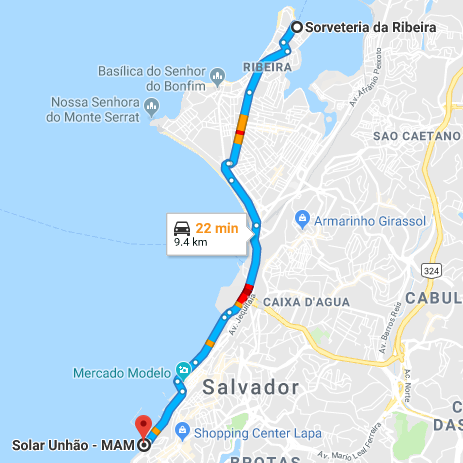
\includegraphics[scale=0.63]{images/image_2018-04-06_01-20-19.png}
	\caption{Rota gerada no Google Maps.}
	\label{fig:route_default}
\end{figure}

\section{Sumário}
\label{sec:summaryIntroduction}

Neste capítulo motiva-se e introduz o problema que este trabalho propõe resolver. Os próximos capítulos estão organizados da seguinte maneira: o capítulo \ref{chp:recSys} apresenta os conceitos teóricos usados neste trabalho referentes a Sistemas de Recomendação. O capítulo \ref{chp:eTourism} apresenta conceitos sobre Sistemas de Recomendação aplicados em Geolocalização. O capítulo \ref{chp:eTourismRecSys} apresenta a proposta de aplicação de sistemas de recomendação baseado em filtragem colaborativa em sugestões de rotas de pontos turísticos, além de discutir como foi feita a implementação. O capítulo \ref{chp:evaluation} apresenta a avaliação da ferramenta, conclusões e considerações finais.
\chapter{Sistemas de Recomendação}
\label{chp:recSys}

\begin{quotation}[]{Autor Desconhecido}
Discipline is doing what you know needs to be done, even if you don't want to do it.
\end{quotation}

A grande quantidade de informação produzida e disponibilizada atualmente pode gerar uma sobrecarga para o usuário. Por causa deste problema, muitas tecnologias surgiram para apoiar a seleção, recuperação e filtragem da informação de interesse do usuário. Este capítulo fornece uma visão geral sobre Sistemas de Recomendação, introduz os principais conceitos em sistemas de recomendação, as tarefas e técnicas que a caracterizam. \newline

\section{Histórico}
\label{sec:historyRecSys}

Os primeiros sistemas de recomendação foram tradicionais sistemas de filtragem e recuperação da informação, os quais não podiam recomendar mais do que certos resultados de acordo com a pesquisa. O primeiro sistema de recomendação foi um sistema experimental de filtragem de e-mail: \textit{Tapestry} \citep{Goldberg:1992:UCF:138859.138867}, desenvolvido por pesquisadores da \textit{Xerox Palo Alto Research Center}. A motivação para o \textit{Tapestry} veio do aumento do número de e-mails que chegavam no centro de pesquisa \citep{Resnick:1997:RS:245108.245121}. \textit{Tapestry} foi elaborado para lidar com filtragem colaborativa - sendo os primeiros a usar o termo - e filtragem baseada em conteúdo. A parte colaborativa do sistema filtra e arquiva os e-mails de acordo com as reações das pessoas que já tinham lido.

Em sua forma mais simples, recomendações personalizadas são fornecidas como listas de itens classificados. Para gerar essa lista, sistemas de recomendação tentam predizer qual produto ou serviço mais se encaixa, baseado nas preferências do usuário. Para isso, eles coletam as preferências do usuário que podem ser expressas explicitamente. Por exemplo, avaliando produtos ou realizando inferências a partir das ações do usuário, o sistema pode considerar um acesso à página de um produto como um sinal implícito de preferência \citep{Ricci:2010:RSH:1941884}.

As pessoas frequentemente dependem de recomendações. seja através de recomendação de amigos, \textit{reviews} de livros e filmes, ou guias de restaurantes. O sistema de recomendação apoia e aumenta esse processo natural \citep{Resnick:1997:RS:245108.245121}. Basicamente, sistemas de recomendação são técnicas e ferramentas de software para fornecer sugestões de itens que sejam úteis para um usuário. Nesses sistemas, \quotes{item} é um termo genérico utilizado para denotar o que o sistema recomenda a um usuário \citep{Ricci:2010:RSH:1941884}.

Sistemas de recomendação são largamente utilizados no comércio eletrônico, entretenimento, consumo de conteúdo, indústria de serviço, entre outros. Esses podem ser encontrados em muitas aplicações modernas que entregam ao usuário uma enorme coleção de itens, recomendando itens ao usuário final utilizando uma combinação de abordagens baseada em conteúdo, filtragem colaborativa e em conhecimento \citep{Ricci:2010:RSH:1941884}. Por exemplo, o serviço de \textit{streaming} de filmes \textit{Netflix}\footnote{https://www.netflix.com} exibe predições de classificação para cada filme exibido, ajudando o usuário a decidir qual filme assistir. A loja online \textit{Amazon}\footnote{http://www.amazon.com/} fornece, na página de um produto, informações de outros produtos comprados por usuários que compraram aquele produto \citep{evaluating-recommender-systems}.

Com o rápido crescimento da quantidade de informação disponível na Web, que frequentemente sobrecarregam o usuário, são tomadas decisões pobres ou erradas. Assim a disponibilidade de escolhas, ao invés de ser um benefício, acaba sendo um problema para o usuário \citep{Ricci:2010:RSH:1941884}. Os sistemas de recomendação oferecem novos itens não visitados anteriormente como produtos, filmes, livros, páginas web, etc, baseados nas preferências do usuário mantidas em seu perfil. Os sistemas de recomendação lidam com esse problema de sobrecarga de informação filtrando itens que podem corresponder aos interesses do usuário. Eles ajudam os usuários filtrando informações irrelevantes quando os usuários pesquisam por alguma informação de interesse \citep{DBLP:journals/corr/abs-1109-0166}.

Critérios como \quotes{individualizada} e \quotes{interessante e útil} diferenciam o sistema de recomendação dos sistemas de recuperação de informação ou motores de busca. Em um motor de busca, o sistema deve retornar tudo o que for correspondente a um termo de pesquisa. Porém, motores de buscas começaram a utilizar técnicas como \ac{rr} (em inglês, \textit{Relevance Feedback} - RF) para introduzir o usuário no processo da busca, permitindo que os mesmos indiquem o que é realmente relevante \citep{Burke2002}.

\section{Conceitos}
\label{sec:conceptsRecSys}

Os dados utilizados pelo sistema de recomendação podem se referir a três tipos de objetos: itens, usuários e relações \citep{Ricci:2010:RSH:1941884}.

\begin{itemize}
	\item{\textbf{Itens}: Itens são os objetos recomendados. Podem ser caracterizados por sua complexidade e por seu valor ou utilidade. O valor de um item pode ser positivo se o item é útil para o usuário, ou negativo se o item é inapropriado e o usuário tomou uma decisão errada ao selecioná-lo. Itens podem ser representados utilizando várias abordagens de representação e informação.}
	
	\item{\textbf{Usuários}: Os usuários do sistema de recomendação podem ter diversos objetivos e características. Para personalizar as recomendações os sistemas de recomendação exploram um conjunto de informações sobre o usuário. Essas informações podem ser estruturadas de várias maneiras, e a seleção de quais informações modelar depende da técnica de recomendação. Usuários também podem ser descritos pelo seus padrões de comportamento, como dados de navegação em um site.}
	
	\item{\textbf{Transações}: Transações são registros de interação entre o usuário e o sistema de recomendação. São como dados de log que armazenam informações importantes geradas durante a interação humano-computador, as quais são úteis para geração de recomendação pelo algoritmo que o sistema está utilizando.}
\end{itemize}

\section{Tarefas de um Sistema de Recomendação}
\label{sec:tasksRecSys}

\cite{Ricci:2010:RSH:1941884} apresentou uma lista das tarefas de um sistema de recomendação baseada nos interesses do criador do sistema de recomendação.

\begin{itemize}
	\item{\textbf{Aumentar o número de itens vendidos}: Essa é, provavelmente, a função mais importante para um sistema de recomendação comercial. Ele deve ser capaz de vender um conjunto de itens adicionais comparado a aqueles que venderiam sem qualquer tipo de recomendação.}
	
	\item{\textbf{Vender mais itens diferentes}: Outra função importante de um sistema de recomendação é possibilitar que o usuário encontre itens que seriam difícil de encontrar sem uma recomendação precisa.}
	
	\item{\textbf{Aumentar a satisfação do usuário}: Uma combinação de recomendações precisas e uma interface bem desenhada irão aumentar a avaliação subjetiva que o usuário tem do sistema. Isso irá aumentar a utilização do sistema e a probabilidade de as recomendações serem aceitas.}
	
	\item{\textbf{Aumentar a fidelidade do usuário}: Um usuário deve ser fiel a um site que reconhece-o como um cliente antigo e trata-o como um visitante de grande valor. Esse é um recurso comum em sistemas de recomendação, já que eles calculam recomendações avaliando as informações adquiridas do usuário em interações anteriores.}
	
	\item{\textbf{Melhor entendimento do que o usuário quer}: A descrição das preferências do usuário, coletadas explicitamente ou preditas pelo sistema, podem ser reutilizadas para vários objetivos.}		
\end{itemize}

\cite{Herlocker:2004:ECF:963770.963772} define onze tarefas de usuário que um sistema de recomendação pode auxiliar a implementar para apoiar o usuário em seus objetivos.

\begin{itemize}
	\item{\textbf{Anotação em contexto}: Dada uma lista de itens em um contexto, destacar alguns deles de acordo com as preferências do usuário.}
		
	\item{\textbf{Encontrar bons itens}: Fornecer ao usuário uma lista ranqueada dos itens recomendados, com uma previsão do quanto o usuário gostará desses itens.}
	
	\item{\textbf{Encontrar todos os bons itens}: Fornecer ao usuário uma lista de todos os itens que podem satisfazer suas necessidades. Em alguns casos encontrar apenas alguns bons itens pode não ser o suficiente. Na prática, o sistema tem que garantir ter uma taxa de "falso negativo"~ suficientemente baixa.}
	
	\item{\textbf{Recomendar uma sequência}: Aqui tem-se o desafio de recomendar uma sequência de itens relacionados.}
	
	\item{\textbf{Recomendar um grupo}: Recomendar um grupo de itens relacionados que possam interessar o usuário.}
	
	\item{\textbf{Apenas navegar}: O sistema deve auxiliar os usuários que apenas navegam sem um propósito definido, navegando entre os itens que possam ser interessantes naquela sessão específica.}
	
	\item{\textbf{Encontrar sistema de recomendação confiável}: Os usuários podem não confiar no sistema de recomendação, assim o sistema deve possibilitar que o usuário teste algumas funções.}
	
	\item{\textbf{Melhorar o perfil}: O sistema deve receber informações do usuário sobre o que ele gosta e não gosta. As contribuições do usuário aperfeiçoarão a qualidade das recomendações.}
	
	\item{\textbf{Expressar-se}: Alguns usuários não se importam com as recomendações, apenas estão interessados em contribuir com as qualificações. Assim, o sistema deve fornecer uma seção para comentários.}
	
	\item{\textbf{Ajudar os outros}: Alguns usuários gostam de contribuir com informação porque eles acreditam que a comunidade se beneficia de sua avaliação.}
	
	\item{\textbf{Influenciar os outros}: Existem ainda usuários maliciosos, que tentarão influenciar outros a escolher um determinado item, ou ainda utilizarão o sistema apenas para promover ou penalizar um item.}
\end{itemize}

\section{Técnicas de Recomendação}
\label{sec:tecnicsRecSys}

Para a realização da recomendação são utilizadas algumas técnicas baseadas em predições. Tais predições podem ser feitas a partir das informações de itens, ou de usuários.

Várias técnicas de recomendação foram propostas como base para um sistema de recomendação, como as técnicas colaborativa, baseada em conteúdo, baseada em conhecimento e demográfica. As técnicas de recomendação podem ser diferenciadas com base em suas fontes de conhecimento, mas existe a indagação de qual a fonte do conhecimento necessário para fazer a recomendação. Em alguns sistemas, esse conhecimento é o conhecimento das preferências de outros usuários \citep{Burke2007}.

A utilidade de um item para um usuário pode ser influenciada pelo conhecimento que o usuário tem do domínio, como um usuário iniciante comparado a um usuário experiente de uma câmera digital. O interesse do usuário pelo item também pode depender do momento em que a recomendação foi feita. Por exemplo, o usuário pode estar mais interessado em um restaurante mais perto de seu local atual. Assim, a recomendação deve ser adaptada para esses detalhes específicos adicionais \citep{Ricci:2010:RSH:1941884}.

\cite{Burke2007} apresentou quatro diferentes classes de técnicas de recomendação baseadas em fontes de conhecimento, como ilustrado na Figura \ref{fig:recommendation_techniques_knowledge_sources}:

\begin{figure}
	\centering
	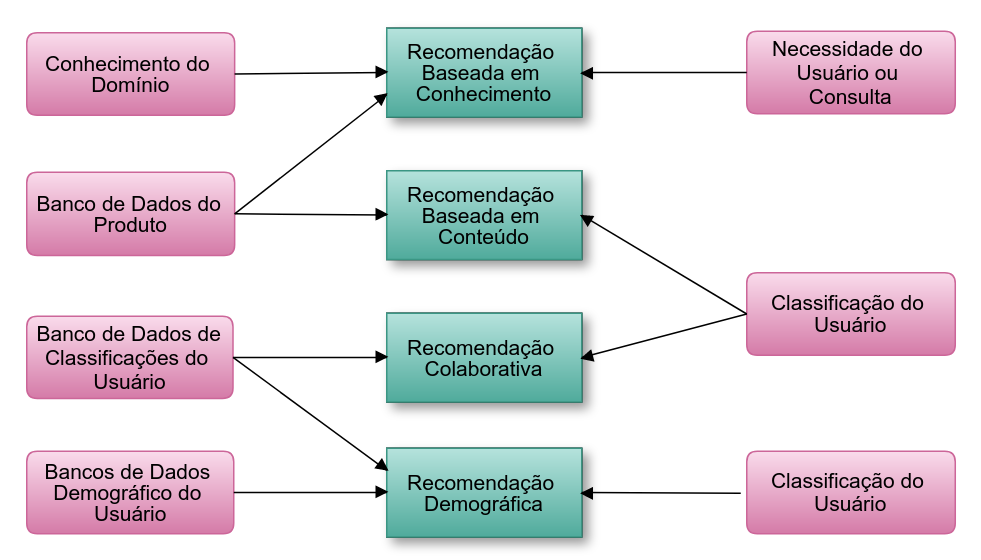
\includegraphics[scale=0.63]{images/recommendation_techniques_knowledge_sources.png}
	\caption{Técnicas de recomendação e suas fontes de conhecimento \citep{Burke2007}.}
	\label{fig:recommendation_techniques_knowledge_sources}
\end{figure}

\begin{itemize}
	\item{\textbf{Filtragem Colaborativa}: O sistema gera recomendações para um usuário utilizando apenas informações de itens de outros usuários com gosto similar.}
	
	\item{\textbf{Baseada em Conteúdo}: O sistema gera recomendação de duas fontes: as características associadas ao item e as classificações que os usuários deram a ele.}
	
	\item{\textbf{Demográfica}: Fornece recomendações baseado no perfil demográfico do usuário.}
	
	\item{\textbf{Baseada em Conhecimento}: Sugere itens baseado em inferências sobre as preferências e necessidades do usuário.}
\end{itemize}

	A seguir é discutido em detalhes alguns dos tipos de recomendação.
	
\subsection{Filtragem Colaborativa}
\label{subsec:cfRecSys}

Na filtragem colaborativa o sistema recomenda ao usuário ativo itens que usuários com gostos similares gostaram no passado. A semelhança de gostos de dois usuários é calculada baseada na similaridade do histórico de classificações dos usuários. A filtragem colaborativa é considerada a técnica em sistemas de recomendação mais popular e mais largamente implementada \citep{Ricci:2010:RSH:1941884}.

A ideia chave é que a classificação de um usuário \textit{u} para um novo item \textit{i} é provável de ser parecido para a de outro usuário \textit{v}, se \textit{u} e \textit{v} tem classificado outros itens de maneira equivalente. De modo similar, é provável que \textit{u} classifique dois itens \textit{i} e \textit{j} de forma semelhante, se outros usuários tem feito classificações similares para estes dois itens \citep{Ricci:2010:RSH:1941884}.

Em \cite{Burke2002} e \cite{Burke2007}, tem-se que os métodos de filtragem colaborativa podem ser divididos nas duas classes gerais baseados em \textit{vizinhança} e \textit{modelo}. Na filtragem colaborativa baseada em vizinhança, as classificações usuário-item armazenadas no sistema são utilizadas diretamente para predizer classificações para novos itens. Isto pode ser feito de duas maneiras conhecidas como recomendação \textit{user-based} ou \textit{item-based} \citep{Ricci:2010:RSH:1941884}.

Sistemas baseados em usuário, avaliam o interesse de um usuário \textit{u} por um item \textit{i} utilizando as classificações, para este item, de outros usuários, chamados \textit{vizinhos}, que tem padrões de classificação similar. Os vizinhos do usuário \textit{u} são tipicamente os usuários \textit{v} cujas classificações para os itens classificados por \textit{u} e \textit{v}, isto é I{$_{uv}$}, são mais correlacionados com aqueles de \textit{u}. A abordagem baseada no item, por outro lado, prediz a classificação de um usuário \textit{u} para um item \textit{i} baseado nas classificações de \textit{u} para itens similares a \textit{i}. Em tais abordagens, dois itens são similares se muitos usuários do sistema tem classificado estes itens de maneira similar \citep{Ricci:2010:RSH:1941884}.

Diferente dos sistemas baseado em vizinhança, que usam as classificações armazenadas diretamente na predição, abordagens baseadas em modelo usam essas classificações para aprender um modelo preditivo. A ideia geral é modelar as interações usuário-item com fatores representando características latentes dos usuários e itens no sistema, como a classe de preferência do usuário e a classe de categoria dos itens. Este modelo é então treinado utilizando os dados disponíveis, e depois utilizado para predizer classificações de usuários para novos itens \citep{Ricci:2010:RSH:1941884}.

\subsection{Filtragem Baseada em Conteúdo}
\label{subsec:contextFilterRecSys}

Sistemas de recomendação baseado em conteúdo tentam recomendar itens similares a aqueles que um usuário gostou no passado, ao passo que sistemas que utilizam o paradigma de recomendação colaborativa identificam usuários que possuem preferências similares a um usuário e recomenda itens que eles tem gostado \citep{Lops2011}.

Sistemas implementando uma abordagem de recomendação baseada em conteúdo analisam um conjunto de documentos e/ou descrições de itens previamente classificados por um usuário, e constroem um modelo ou perfil de interesses do usuário baseado nas características dos objetos classificados por este usuário \citep{784084}. O perfil é uma representação estruturada dos interesses do usuário, adaptado para recomendar novos itens interessantes. O processo de recomendação consiste basicamente em combinar os atributos do perfil do usuário contra os atributos de um objeto de conteúdo. O resultado é um julgamento de relevância que representa os níveis de interesse do usuário naquele objeto. Se um perfil reflete com precisão as preferências do usuário, isso é uma grande vantagem para a eficácia no processo de acesso a informação. Por exemplo, um perfil pode ser utilizado para filtrar os resultados de pesquisa para decidir se um usuário está interessado em uma específica página Web ou não e, em caso negativo, prevenir de ser exibida \citep{Lops2011}.

\subsection{Arquitetura de Sistemas de Recomendação Baseados em Conteúdo}
\label{subsec:cb-recsys-architecture}

Segundo \cite{Lops2011}, em sistemas baseados em conteúdo é necessário utilizar técnicas apropriadas para representar os itens e produzir o perfil do usuário, além de algumas estratégias para comparar o perfil do usuário com a representação do item. O processo de recomendação é realizado em três passos, cada qual é manipulado por um componente separado:

\begin{itemize}
	\item{\textbf{Analisador de Conteúdo}: Quando a informação não tem estrutura, como um texto, algum tipo de pré-processamento é preciso para extrair informação relevante e estruturada. A principal responsabilidade do componente é representar o conteúdo dos itens (por exemplo, documentos, páginas Web, notícias, descrição de produtos, etc.) vindos de fontes de informação de forma adequada para o próximo passo de processamento.}
	
	\item{\textbf{Aprendiz de Perfil}: Este módulo coleta dados representativos das preferências dos usuários e tenta generalizar estes dados, para construir o perfil do usuário. Normalmente, a estratégia de generalização é realizada através de técnicas de \textit{aprendizado de máquina}, que são capazes de inferir um modelo de interesses de usuário partindo de itens gostados ou não gostados no passado.}
	
	\item{\textbf{Componente de Filtragem}: Este módulo explora o perfil do usuário para sugerir itens relevantes através da combinação da representação do perfil do usuário contra os itens a serem recomendados. O resultado é um binário ou contínuo julgamento de relevância (computado utilizando alguma métrica de similaridade \citep{Herlocker:2004:ECF:963770.963772}), neste último caso resultando em uma lista ranqueada de itens potencialmente interessantes.}
\end{itemize}

A arquitetura de alto nível de um sistema de recomendação baseado em conteúdo está retratada na Figura \ref{fig:high_level_arch_content_based_rec_order}.

\begin{figure}
	\centering
	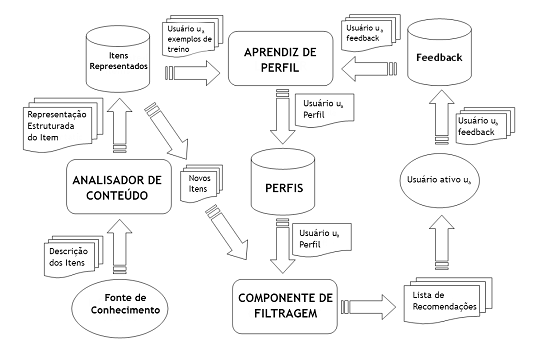
\includegraphics[scale=0.88]{images/high_level_arch_content_based_rec_order.png}
	\caption{Arquitetura de alto nível de um Sistema de Recomendação Baseado em Conteúdo \citep{Lops2011}.}
	\label{fig:high_level_arch_content_based_rec_order}
\end{figure} 


\subsection{Comparação das Técnicas de Recomendação}
\label{subs:compareRecTech}

Todas as técnicas de recomendação tem seus pontos fortes e fracos. \cite{Burke2002} indicou alguns desses pontos, os quais são discutidos abaixo:

\begin{itemize}
	\item{\textbf{Usuário Novo}: Recomendações partem da comparação entre o usuário alvo e outros usuários baseando-se unicamente na acumulação de classificações. Dessa forma um usuário com poucas classificações é difícil de categorizar.}
	
	\item{\textbf{Item Novo}: Do mesmo modo, um item novo que não tem recebido muitas classificações também não pode ser facilmente recomendado: o problema do "item novo". É também conhecido como problema do "early rater", desde que a primeira pessoa a classificar um item recebe poucos benefícios por fazer isso. Isso torna necessário que sistemas de recomendação forneçam outros incentivos para encorajar usuários a fornecer classificações.}
\end{itemize}

Sistemas de recomendação colaborativos dependem das recomendações entre usuários e tem problemas quando o espaço de classificações é esparso, na qual poucos usuários classificam os mesmos itens. Estes problemas sugerem que técnicas colaborativas puras são melhores para problemas em que a densidade de interesse do usuário é relativamente alta entre um pequeno e estático universo de itens. Se o conjunto de itens muda rapidamente, classificações antigas serão de pouco valor para novos usuários que não serão capazes de ter suas classificações comparadas com as dos usuários existentes. Se o conjunto de itens é grande e o interesse do usuário dissemina pouco, então a probabilidade de sobreposição com outros usuários será pequena \citep{Burke2002}.

Sistemas de recomendação colaborativos funcionam melhor para um usuário que se encaixa em um nicho com muitos vizinhos de gosto semelhante. A técnica não funciona bem para o chamado "\textit{gray sheep}"~ \citep{claypool99}, que cai na fronteira entre panelinhas de usuários existentes. Isso também é um problema para sistemas demográficos que tentam categorizar usuários em características pessoais. Por outro lado, sistemas de recomendação demográficos não tem o problema do "usuário novo", porque eles não requerem um lista de classificações dos usuários. Ao invés, eles tem o problema de reunir as informações demográficas necessárias. \citep{Burke2002}.


\section{Sumário}
\label{sec:summaryRecSys}

Neste capítulo foi apresentado uma visão geral sobre os Sistemas de Recomendação. Primeiramente mostrando um histórico sobre Sistemas de Recomendação. Em seguida, é discutido alguns conceitos sobre os dados utilizados em um sistema, além das principais técnicas de recomendação. Então, foi apresentado uma lista de tarefas desempenhadas por sistemas de recomendação. No capítulo seguinte será discutido sobre Sistemas de Recomendação \textit{e-Tourism}, introduzido do que se trata, formas e requisitos de modelagem e algumas aplicações de sistemas de recomendação.
\chapter{\textit{e-Tourism}}
\label{chp:eTourism}

O turismo é um setor de grande importância e que está sofrendo modificações com a inserção do comércio eletrônico como ferramenta para a realização de negócios. No Brasil, os dados de 2016 são: 6,6 milhões de turistas estrangeiros; 90,3 milhões de turistas nacionais; US\$ 6 bilhões de receitas diretas com o turismo interno. Segundo a mesma fonte, em 2015 houve US\$ 1.194 bilhões de receita cambial no turismo mundial \citep{embratur2016}.

Com a facilidade de acesso a rede e a ascensão dos dispositivos móveis, é cada vez mais necessário o desenvolvimento de sistemas que utilizem os recursos de mobilidade e de acesso à informação turística a qualquer hora e lugar. Nessa sessão, apresenta-se os principais conceitos envolvidos no trabalho e descrever trabalhos relacionados a sistemas de recomendações voltadas ao turismo.

\section{Introdução}
\label{sec:introductionETourism}

O avanço das tecnologias móveis e da Internet no nosso dia-a-dia vieram como uma maneira de revolucionar o comércio de produtos e serviços, permitindo rapidez e facilidade na hora de fazer uma compra, reduzindo os custos e o tempo. Isso modificou, de uma maneira geral, os mercados, seja de livros, músicas e jogos até entretenimento, como viagens, esportes, entre outros.

O comércio eletrônico revolucionou o anúncio, a distribuição, a venda e a informação de produtos turísticos, fazendo com que surgissem diversos sites especializados em turismo, seja para divulgar informações sobre bares, restaurantes, pontos turísticos e atrações das cidades, seja para facilitar na compra e venda de viagens, reserva de passagens, pousadas, hotéis e no transporte coletivo \citep{115416147001}. Diante dos números apresentados anteriormente, a Internet é uma ferramenta importante, pois contribui para a escolha de roteiros turísticos, representando investimento de tempo e dinheiro. Logo, o acesso as informações precisas e confiáveis são fundamentais para orientar o turista na escolha adequada \citep{115416147001}.

O turismo é uma atividade fortemente conectada com preferências pessoais e interesses das pessoas \citep{4669760}. Pensando nisso, o \textit{e-Tourism} vem como a possibilidade de personalizar a filtragem de informações, sugerindo ao usuário locais que são do interesse do mesmo, de acordo com suas preferências e outras variáveis (tempo disponível, programa para família ou individual, entre outros). \textit{e-Tourism} ou turismo eletrônico é definido como a digitalização de todos os processos e cadeias de valor da indústria do turismo, viagens, hotelaria e restauração que permitem às organizações maximizar sua eficiência e sua eficácia \citep{Moura:2013:DUT:2526188.2526215}.

\section{Sistemas de Informação para \textit{e-Tourism} e Classificações}
\label{sec:eTourism_infosys_classification}

Atualmente, muitas pessoas que planejam uma viagem procuram primeiramente a Internet para saber mais informações do local que pretendem visitar e programar suas as atividades. A Internet e as demais tecnologias tem facilitado bastante a vida das pessoas antes de uma viagem. Porém o visitante tem pouco conhecimento da cidade que irá visitar, além de não conhecer algumas atrações e os pontos turísticos que a cidade tem. Além disso, o usuário perde tempo para selecionar as atividades de sua preferência que ele pode fazer na cidade e organizá-los de forma que aproveite melhor o tempo disponível na viagem.

\subsection{Sistemas de Informação}
\label{subsec:eTourism_infoSys}

Existem diversos sistemas que disponibilizam informações de acordo com a entrada de preferências do usuário, entre eles os mais utilizados:

\begin{itemize}
    \item TripAdvisor\footnote{https://www.tripadvisor.com/}: é um site de turismo que auxilia em viagens, cidades para visitação e atividades para cada usuário e que também contém uma rede social, sendo possível adicionar \textit{reviews}, comentar e pontuar, ajudando no processo de tomada de decisões que pertence ao domínio do turismo.
    \item Booking.com\footnote{https://www.booking.com/}: site \textit{e-commerce} de viagens no mundo. Permite que você possa encontrar e reservar de uma maneira mais rápida a pousada ou hotel para a próxima viagem. Como diferencial, é possível procurar por hotéis próximos a localização ou próximo ao local que o usuário desejar. Por exemplo, se o turista está indo para a cidade de São Paulo, pode-se localizar hotéis próximos ao centro da cidade, ou ao Parque de Ibirapuera, entre outros.
    \item Foursquare\footnote{https://foursquare.com/}: uma rede social que ajuda de encontrar novas maneiras de explorar a cidade de acordo com as preferências de cada usuário. É possível fazer o \textit{check-in} da localização atual, classificar e deixar \textit{reviews} de locais.
\end{itemize}

\subsection{Classificação}
\label{subsec:eTourism_classification}

Encontram-se diversas formas de classificar os sistemas de recomendação para \textit{e-Tourism} \citep{BORRAS20147370}: pelas interfaces e por funcionalidades. A seguir, é discutido de forma mais detalhada como é feita essa classificação.

\subsubsection{Interfaces}
\label{subsubsec:eTourism_classification_interfaces}

A maioria dos sistemas de recomendação para turismo oferecem uma interface Web e/ou interface para dispositivos móveis. A interface Web permite que o usuário tenha uma maior interação com o sistema, visualizando as informações em mapas interativos, imagens e/ou vídeos de alta qualidade.  Como exemplo, o \textit{e-Tourism} \citep{4669760} mostra em um mapa os locais para serem visitados em um dia, de acordo com a programação.
Já o mobile permite que o usuário possa acessar as informações de qualquer lugar e utilizar de ferramentas que os dispositivos oferecem para incrementar o sistema na recomendação de locais para visitação (por exemplo, utilizar o GPS para saber da localização do turista e mostrar informações de pontos próximos a ele). O projeto \textit{ReRex} serviço que recomenda POIs para usuários mobile. \citep{Baltrunas2012}. Já o \textit{MTRS} \citep{Gavalas2011} é um sistema mobile que permite aos turistas construir roteiros customizados e oferece informações turísticas.

\subsubsection{Funcionalidades}
\label{subsubsec:eTourism_classification_functionalities}

Cada sistema de recomendação de turismo oferece diversas utilidades para o turista. Os mais comuns são:

\begin{itemize}
    \item Sugestão de destino e/ou construção de pacotes de turismo. O sistema tem como foco a recomendação de destinos que respeitem as preferências do usuário. No \textit{MyTravelPal} \citep{article} o turista é capaz de interagir em um mapa, no qual o sistema recomenda áreas de interesse na região. O tamanho do círculo indica o grau de afinidade com o usuário (Figura \ref{fig:recommended_municipalities}). Com foco em uma determinada área, é possível visualizar todos os locais e o tamanho depende da afinidade do perfil do viajante (Figura \ref{fig:recommended_tourist_objects}).
    \item Lista de classificação de atrações sugeridas: a maioria dos sistemas de recomendação de turismo fazem sugestões de pontos turísticos para o usuário que já decidiu para qual cidade viajará ou se ele já foi em um determinado local. Nesse caso, a classificação e pontuação dos pontos turísticos são de extrema importância para o sistema que tem disponível uma grande quantidade de informações para ser processada de acordo com as particularidades do usuário. Mais uma vez, o \textit{e-Tourism} \citep{4669760} é um bom exemplo de sistema de recomendação que utiliza uma lista de atividades que usuário deseja realizar, aquelas que já realizou além de locais que o turista já foi anteriormente.
    \item Planejamento de rotas: como já diz, sistemas desse tipo ajudam a criar rotas com uma lista de lugares de acordo com as preferências do turista. Para exemplificar o protótipo de \cite{Moura:2013:DUT:2526188.2526215} tem como foco traçar um itinerário no roteiro Caminhos da Pedra, na cidade de Bento Gonçalves, em que as atrações melhor avaliadas e relacionadas com os contextos do usuário possam ganhar mais visibilidade.
    \item Aspectos sociais. O sistema permite que os usuários compartilhem fotos, comentários, adicionarem uma pontuação ao local e interajam com outros turistas. Com isso, é possível recomendar locais analisando o \textit{score} e os comentários dos outros visitantes. O projeto \textit{e-Tourism} \citep{4669760} é um exemplo, que permite criar planos para visitação de locais de acordo com as preferências de um grupo de visitantes.
\end{itemize}

\begin{figure}
	\centering
	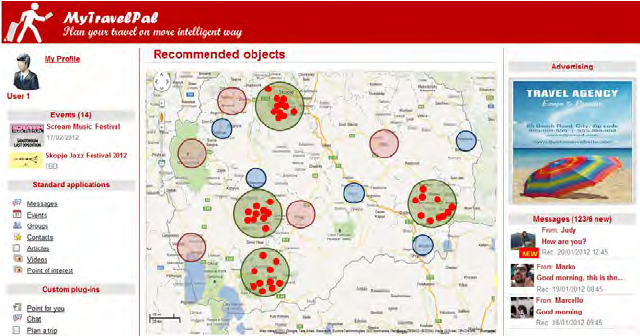
\includegraphics[scale=0.7]{images/Figure-no-1-Screenshots-of-the-recommended-municipalities.png}
	\caption{\textit{MyTravelPal}: mapa com recomendação de áreas de interesse \citep{article}.}
	\label{fig:recommended_municipalities}
\end{figure}

\begin{figure}
	\centering
	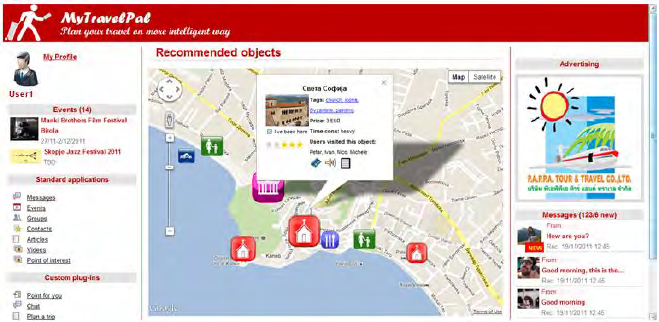
\includegraphics[scale=0.7]{images/Figure-no-2-Screenshots-of-recommended-tourist-objects.png}
	\caption{\textit{MyTravelPal}: mapa com recomendação de pontos turísticos e suas informações \citep{article}.}
	\label{fig:recommended_tourist_objects}
\end{figure}

\section{Sistemas de Recomendação para \textit{e-Tourism}}
\label{sec:eTourism_recsys}

Os sistemas de recomendação para turismo trazem pontos turísticos com base na individualidade de cada viajante. Cada sistema trabalha de uma maneira diferente na sugestão dos locais para o turista. Será apresentado três tipos de sistemas de recomendação para \textit{e-Tourism}: baseado em experiência de usuário, pontos de interesse e baseado em rotas.

\subsection{Sistemas de Recomendação Baseado em Experiência de Usuário}
\label{subsec:eTourism_recsys_userXP}

Os sistemas de recomendação baseados em experiência do usuário para \textit{e-Tourism} primeiramente verificam quais foram os pontos turísticos que o usuário já visitou antes, seja na cidade que ele deseja visitar, seja no histórico geral do turista, ou seja, pré-classificar alguns itens \citep{BORRAS20147370}. Com isso, é possível definir um gosto comum e, com essas informações, o sistema constrói um perfil inicial. 

Primeiramente, o sistema sugere locais que são parecidos com o que ele já visitou e o usuário marca as atrações do seu agrado e desmarca aquelas que ele não aprovou. Após a visita do turista nas atrações, este pode opinar deixando um \textit{feedback} ou uma pontuação sobre o local. O processamento do \textit{feedback} do usuário é muito importante pois é através das informações obtidas das suas avaliações que o sistema de recomendação melhora o perfil do turista e pode oferecer pontos que mais se adaptam ao seu gosto \citep{4669760}.

Um exemplo disso é o \textit{e-Tourism}, um sistema que constrói um itinerário de acordo algumas características e restrições do usuário para a visita, como o período, o tempo destinado para a visitação, se estará sozinho ou com a família, além do local de origem, idade e gênero \citep{4669760}.

\subsection{Sistemas de Recomendação de Pontos de Interesse}
\label{subsec:eTourism_recSys_poi}

O rápido crescimento e desenvolvimento das cidades proporcionou um número muito grande de pontos de interesse (conhecido na língua inglesa como \ac{poi}), como por exemplo restaurantes, hotéis, lojas, entre outros. Diante de uma larga quantidade de POIs, o usuário tem problemas de fazer uma decisão satisfatória de "onde ir" de acordo com seus interesses pessoais. Sistemas de Recomendação de Pontos de Interesse tem como objetivo resolver um destes problemas ajudando os usuários a filtrar os POIs mais importantes e reduzir o tempo gasto para fazer uma decisão \citep{AAAI159560}.

O desenvolvimento de redes sociais baseada em localização (\ac{lbsn}) permite que sistemas de recomendação de POIs em LBSNs possam estudar os comportamentos do usuário mobile para recomendação de POIs de acordo com aspectos de espaço, de tempo, sociais e de conteúdo. Através dos \textit{check-ins} dos usuários nas redes sociais de geolocalização utilizando \textit{smartphones}, é possível visualizar quem, quando, onde e o que foi marcado como ponto de interesse \citep{AAAI159560}.

As informações contidas nos LBSNs pode estar relacionados a ação de \textit{check-in} do usuário, promovendo uma única oportunidade para sistemas de recomendação baseadas em POIs. Como exemplo, verificando a descrição de um POI que contém "churrascaria", conclui-se que este restaurante tem como prato principal carnes vermelhas e usuários que fazem \textit{check-in} neste POI talvez tenham interesse em churrasco. Este é um exemplo de propriedade de POI. Isso mostra que recomendações de POIs para um usuário baseado nas suas ações através de \textit{check-ins} leva em consideração as informações disponíveis, como exemplo, interesses do usuário e propriedades de POIs.

O \textit{framework} desenvolvido em \cite{AAAI159560} para recomendação de pontos de interesse leva em conta também indicações de sentimento do usuário no POI. No exemplo anterior, o POI da churrascaria pode conter comentários de diversos usuários sobre o local, elogiando ou deixando uma reclamação, seja da comida ou do serviço prestado pelo estabelecimento. Nessa pesquisa, foi utilizado os \textit{check-ins} da rede social \textit{Foursquare}\footnote{http://sendible.com/insights/what-is-foursquare-location-based-social-networking}, uma das mais populares LBSN.

Em muitos sistemas de recomendação baseado em filtragem colaborativa utilizando POIs, são considerados somente os pontos de interesse que o usuário ou seus amigos já visitaram, não funcionando corretamente quando inclui pontos que anda não foi visitados. Para contornar esse problema, \cite{Ying:2012:UPR:2346496.2346507}, propôs o \textit{Urban POI-Mine (UPOI-Mine)}, que tem como objetivo criar um sistema de recomendações baseado em filtragem colaborativa utilizando POIs. Foram utilizados três aspectos complementares para extrair características dos POIs dos usuários: fator social, preferencia individual e popularidade do POI.

O aspecto fator social corresponde a oferecer POIs para o usuário de acordo com todos os \textit{check-ins} entre os seus amigos que contém preferências similares, considerando análises estatísticas. As preferências individuais capturam relações entre usuários e POIs, explorando as atividades de \textit{check-ins} do usuário para pontos de interesse com as mesmas propriedades. Porém, esses dois aspectos podem não funcionar corretamente para novos usuários pois informações de \textit{check-ins} são bem escassas. A popularidade dos POIs é incluída para maximizar a estimativa de semelhança da relação entre usuário e POI. Por exemplo, pessoas podem ir todos os dias a uma churrascaria, mas raramente vão a um restaurante oriental. Pensando assim, estima-se a equivalência por probabilidade condicional, que é a probabilidade de os usuários irem a um determinado ponto, de acordo com a categoria. Isto é chamado de popularidade relativa do POI.

Um outro exemplo é o de \cite{Ye:2011:EGI:2009916.2009962}, que além de utilizar a influência social dos amigos do usuário, utiliza-se também a influencia geográfica. \cite{Ye:2011:EGI:2009916.2009962} verificou que os usuários tendem a visitar POIs próximos, seja do trabalho ou de casa, ou de um ponto que esteja próximo da sua atual localização, mesmo que seja longe de casa. Essa análise impactou mais na recomendação de pontos de interesse em LBSNs comparado com a influência social.

\subsection{Sistemas de Recomendação Baseado em Rotas}
\label{subsec:eTourism_recSys_routes}

Existem diversas ferramentas de navegação e transporte que oferecem serviços de rotas baseados na localização do usuário. Como exemplo o \textit{Google Maps}\footnote{https://maps.google.com} extrai a localização através do GPS do celular ou utilizando tecnologias alternativas. Essa é uma das principais características de um sistema de recomendação baseado em rotas: construir uma rota capaz de atender as necessidades do usuário com diferentes focos \citep{GAVALAS2014319}.

Um dos focos é oferecer a menor rota de POIs recomendados próximos da atual localização do usuário. É possível utilizar informações de redes sociais (com \textit{tags} e pontuações colaborativas) para providenciar recomendações de rotas personalizadas \citep{GAVALAS2014319}. Outro ponto são passeios turísticos personalizados, como exemplo, lista ordenada de atrações ao longo de um ponto de origem e destino, de acordo com as preferências do usuário e outras variáveis: atual posição do turista, tempo disponível, interesses de viagem, passeios a pé personalizados, entre outros \citep{GAVALAS2014319}.

Mais um foco são sistemas de recomendação baseado em rotas que englobam meios de transporte, considerando todos os serviços disponíveis na cidade, como metrô, ônibus, a pé, bicicleta, trem, etc. Para isso, o sistema pode criar rotas que utilizam diversos meios de transporte através de um conjunto de POIs ou primeiro gerar o passeio turístico e depois gerar a rota considerando as conduções disponíveis \citep{GAVALAS2014319}. Como exemplo, o UbibusRoute é um sistema móvel que considera informações contextuais dinâmicas do trânsito através de redes sociais, apresentando dados sobre as rotas de ônibus aos usuários \citep{lima2012ubibusroute}.

\begin{table}[h!]
    \centering
	\caption{Análise dos sistemas de recomendação \textit{e-Tourism}.}
	\label{tab:analise_tourism_recommender}
	\begin{tabular}{|r|p{11cm}|}
		\hline
		\multicolumn{1}{|c|}{\bfseries Característica} & \multicolumn{1}{|c|}{\bfseries Referências} \\ \hline
		
		Interface & \cite{4669760}, \cite{Baltrunas2012}, \cite{Gavalas2011}. \\ \hline
		Funcionalidades & \cite{article}, \cite{4669760}, \cite{Moura:2013:DUT:2526188.2526215}. \\ \hline
		Experiência de Usuário & \cite{4669760}.	\\ \hline
		Pontos de Interesse & \cite{AAAI159560}, \cite{Ying:2012:UPR:2346496.2346507}, \cite{Ye:2011:EGI:2009916.2009962}, \cite{Gavalas2011}, \cite{Baltrunas2012}. \\ \hline
		Rotas & \cite{lima2012ubibusroute}, \cite{Moura:2013:DUT:2526188.2526215}. \\ \hline

	\end{tabular}
\end{table}

\section{Sumário}
\label{sec:summaryETourism}

Neste capítulo introduziu-se o \textit{e-Tourism}, mostrando suas aplicações e características. A Tabela \ref{tab:analise_tourism_recommender} mostra um resumo dos sistemas de recomendação de turismo citadas neste capítulo e suas devidas características, classificadas de acordo com as categorias apresentadas anteriormente. Os próximos capítulos estão organizados da seguinte maneira: O Capítulo \ref{chp:eTourismRecSys} apresenta a proposta de aplicação de sistemas de recomendação baseado em filtragem colaborativa em sugestões de rotas de pontos turísticos e discute como foi feita a implementação. O Capítulo \ref{chp:evaluation} apresenta a avaliação da ferramenta e no Capítulo \ref{chp:conclusion} conclusões e considerações finais.
\chapter{Sistema de Recomendação de Rotas de Pontos Turísticos Baseado em Filtragem Colaborativa}
\label{chp:eTourismRecSys}

Para que um software seja desenvolvido de forma consistente, é necessário aliar boas práticas da engenharia de software com um robusto e eficiente processo de desenvolvimento. Neste capítulo, é mostrada as ferramentas utilizadas neste projeto, discutindo seus objetivos e funcionalidades no sistema.
% Um processo de software é um conjunto de atividades que leva ao desenvolvimento do produto. O processo define quem faz, o que faz e quando fazer mas nem sempre diz como fazer. O desenvolvedor ou a organização desenvolve seus próprios processos, significando que não existe um processo ideal \citep{Sommerville2010}. 

\section{Requisitos}
\label{sec:requirements}

% Os requisitos de software são detalhes do que o sistema realizará, os serviços que fornece e as restrições em sua operação \citep{Sommerville2010}. 
O objetivo dessa fase é reunir informações sobre o problema a ser resolvido, de acordo com o que é proposto nesse trabalho. Nessa seção, são detalhados os requisitos do sistema desenvolvido como proposta deste trabalho, fornecendo informações necessárias para o projeto e implementação. Os requisitos de software são classificados como requisitos funcionais e requisitos não funcionais.

% \begin{enumerate}
%     \item \textbf{Requisitos funcionais}: descrevem explicitamente as funcionalidades e os serviços do sistema. Documenta como o sistema deve reagir a entradas específicas, como deve se comportar em determinadas situações e o que o sistema não deve fazer \citep{Sommerville2010}.
%     \item \textbf{Requisitos não funcionais}: definem propriedades e restrições do sistema, podem ser do todo ou parte do sistema. Este tipo de requisito pode ser mais crítico que os requisitos funcionais:se não satisfaz, o sistema é inútil \citep{Sommerville2010}. 
% \end{enumerate}

\subsection{Requisitos Funcionais e Não Funcionais}
\label{subsec:functional_requirements}

Na identificação dos requisitos, foram utilizadas as seguintes convenções: [FRXX] para requisitos funcionais e [NFRXX] para os requisitos não funcionais. São dadas prioridades aos requisitos, que servem para indicar a relevância do requisito para o sistema proposto. Essas são classificadas em: 

\begin{enumerate}
    \item \textbf{Básica}: são requisitos que devem ser implementados. Caso não sejam realizados, o sistema não pode funcionar ou não atende o objetivo da proposta.
    \item \textbf{Significativo}: são requisitos que o sistema pode funcionar, porém de forma parcial.
    \item \textbf{Relevante}: estes requisitos não comprometem o funcionamento básico do sistema; podem ser deixados para versões posteriores deste trabalho.
\end{enumerate}

A Tabela \ref{tab:functional_requirements} apresenta os requisitos funcionais do sistema e a Tabela \ref{tab:non-functional_requirement} apresenta os requisitos não funcionais do sistema, classificados por suas características.

\begin{table}[H]
    \centering
    \begin{tabular}{|c|p{4.5cm}|p{6.5cm}|c|}
        \hline
		
		\multicolumn{1}{|c|}{\bfseries Código} & \multicolumn{1}{c|}{\bfseries Nome} & \multicolumn{1}{c|}{\bfseries Descrição} & \multicolumn{1}{c|}{\bfseries Prioridade} \\ \hline
		
        FR01 & Realizar recomendações de pontos turísticos & Mostrar sugestões de locais para visitação & Básica \\ \hline
        FR02 & Gerar rotas para o usuário & Gerar rotas de acordo com os pontos recomendados pelo sistema, considerando origem e destino do usuário & Básica \\ \hline
        FR03 & Realizar pontos turísticos com base nas informações do usuário & De acordo com as preferências prévias do usuário de outros pontos de localização, gerar recomendações de pontos de acordo com as informações do usuário & Significativo \\ \hline
        FR04 & Gerar a rota com a menor distância para o usuário & Com os resultados obtidos no sistema de recomendação, gerar a menor rota para o usuário & Relevante \\ \hline
        FR05 & Gerar a rota com a menor distância e a maior quantidade de pontos para o usuário & Fornecer ao turista uma rota com a menor distância e com a maior quantidade de pontos de interesses, de acordo com resultados do sistema de recomendação & Relevante\\ \hline
        FR06 & Realizar recomendações, considerando os pontos de origem e destino do usuário & De acordo com a localização do usuário e o destino final da sua rota, considerar o atributo distância na recomendação de pontos & Relevante \\ \hline
    \end{tabular}
    \caption{Requisitos Funcionais do Sistema.}
    \label{tab:functional_requirements}
\end{table}

\begin{table}[H]
    \centering
    \begin{tabular}{|c|p{8.3cm}|c|c|}
        \hline
		
		\multicolumn{1}{|c|}{\bfseries Código} & \multicolumn{1}{c|}{\bfseries Descrição} & \multicolumn{1}{c|}{\bfseries Característica} & \multicolumn{1}{c|}{\bfseries Prioridade}
		\\ \hline
		
        NFR01 & O sistema deve mostrar a rota gerada de uma forma fácil e simples de usar, sem a necessidade de manuais ou treinamento & Usabilidade & Básica \\ \hline
        NFR02 & O sistema deve recomendar pontos turísticos com veracidade & Corretude & Significativo \\ \hline
        NFR03 & O sistema deve gerar rotas seguras dos pontos turísticos recomendados & Corretude & Significativo \\ \hline
        NFR04 & O sistema deve recomendar os pontos turísticos e gerar a rota de uma maneira rápida & Eficiência & Significativo \\ \hline
    \end{tabular}
    \caption{Requisitos Não Funcionais do Sistema.}
    \label{tab:non-functional_requirement}
\end{table}

\section{Arquitetura}
\label{sec:architecture}

Conforme \cite{Bass:2012:SAP:2392670}, arquitetura de software de um programa ou sistema operacional é a estrutura ou estruturas do sistema, que abrange os componentes de software, as propriedades externamente visíveis desses componentes e as relações entre eles.

% Neste projeto, a aplicação foi desenvolvida utilizando o padrão \textit{pipe and filter} (duto e filtro, em português), onde é um modelo no qual as transformações funcionais processam suas entradas e produzem saídas \citep{Sommerville2010}. Neste padrão, o processamento dos dados em um sistema está organizado de modo que cada componente de processamento, chamado filtro, seja discreto. Os dados fluem (como em um duto) de um componente para outro para processamento \citep{Sommerville2010}. 

A Figura \ref{fig:Tourisys_pipe_filter} mostra a arquitetura \textit{pipe and filter} (duto e filtro, em português) para este trabalho. Cada componente (na figura, representados pelos quadrados) age como filtro, realizando as validações dos conteúdos obtidos, transformações e processamentos de dados. Entre um filtro e outro, existem os canais, que agem como dutos.

\begin{figure}[H]
    \centering
    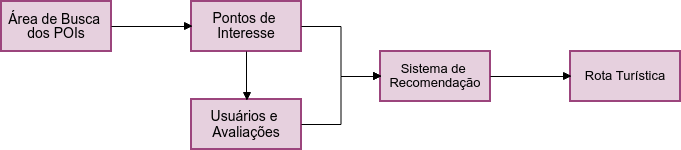
\includegraphics[width=\textwidth]{images/Tourisys_Pipe_Filter.png}
    \caption{Arquitetura do projeto}
    \label{fig:Tourisys_pipe_filter}
\end{figure}

\section{Tecnologias}
\label{sec:technologies}

Para o desenvolvimento do sistema foram utilizadas diversas tecnologias: linguagens de programação, \textit{frameworks}, entre outras. A seguir são apresentadas essas tecnologias.

\subsection{HTML/CSS/JavaScript}

HTML\footnote{https://www.w3.org/html} é uma linguagem de marcação padrão para criar páginas Web. Sua sigla vem do inglês, que significa \textit{HyperText Markup Language}, que significa Linguagem de Marcação de Hipertexto. O HTML é uma linguagem para publicação de conteúdo (texto, imagem, vídeo, áudio etc.) na Web \citep{w3cHTML}. Ela foi utilizada para construir as páginas com as rotas dos pontos turísticos recomendados, que possibilitam a interação do usuário com o sistema.

\textit{Cascading Style Sheets}, mais conhecido como CSS\footnote{https://developer.mozilla.org/en-US/docs/Web/CSS} é uma linguagem de estilo utilizada para descrever a apresentação de um documento escrito em HTML e como os elementos devem ser renderizadas na tela ou em outros meios de comunicação. A tecnologia \textit{JavaScript} (JS)\footnote{https://developer.mozilla.org/bm/docs/Web/JavaScript} é uma linguagem de programação interpretada. Muito conhecida como uma linguagem voltada para páginas Web, a utilização de JS está sendo expandida para outros ambientes. Por exemplo, desenvolvimento de jogos, interfaces para sistemas operacionais, aplicações mobile, banco de dados, entre outros.

\subsection{Python/GraphLab}

Python\footnote{https://www.python.org/} é uma linguagem de programação interpretada, interativa e orientada a objetos. Foi lançada em 1991 por Guido van Rossum. Está disponível para as mais diversas plataformas, incluindo consoles de jogos eletrônicos ou alguns celulares. Caso o sistema operacional não suporte, é possível compilar a partir do código fonte através de um compilador C. Ao longo do tempo, vem sendo desenvolvidas muitas bibliotecas de funções especializadas que permitem expandir as capacidades base da linguagem.
Uma das bibliotecas utilizadas neste trabalho é a GraphLab Create\footnote{https://turi.com/}. É um pacote que permite realizar análise de dados em larga escala. Inclui diversas ferramentas para o desenvolvimento de modelos preditivos de aprendizagem de máquinas e sistemas de recomendação, além da exploração e a visualização de dados.

\subsection{OpenStreetMap/Overpass API}

OpenStreetMap\footnote{http://www.openstreetmap.org} é projeto de produção colaborativa de dados geo-espaciais abertos. Qualquer pessoa pode contribuir e editar o mapa, mantendo atualizadas as informações sobre estradas, pontos de interesses, trilhas, meios de transportes, entre outros, ao redor do mundo. Utilizando informações do OpenStreetMap, o Overpass API\footnote{http://overpass-api.de/} é um serviço que é possível obter informações personalizadas dos dados do mapa do OpenStreetMap. Através dessa ferramenta são obtidos os pontos de interesses relacionado ao turismo com as suas respectivas informações, como nome, descrição, horário de funcionamento, latitude e longitude. Atua como um banco de dados na Web: o cliente envia uma consulta para a API e tem como resultado o conjunto de dados que corresponde à consulta.

\subsection{Google Maps API}

A API\footnote{https://developers.google.com/maps/} do Google Maps é uma plataforma que permite criação de mapas de diferentes tipos (satélite, terreno, entre outros) e com locais definidos, controle de zoom, geração de rotas, pesquisa por estabelecimentos, e outras coisas.
Em nossa pesquisa, essa ferramenta é utilizada para obter informações atualizadas sobre os pontos de localização que estão cadastrados na plataforma, além das avaliações dos usuários do local específico (Google Places API\footnote{https://developers.google.com/places/web-service/}).

\section{Funcionamento}
\label{sec:operation}

A princípio utiliza-se informações dos pontos de interesses obtidos através do OpenStreetMap. Com base nessas informações, são obtidas as avaliações dos usuários que estão registradas no Google Maps. A Figura \ref{fig:tourisys_operation} mostra um fluxograma com uma visão geral do funcionamento do sistema.

Inicialmente (passo 1 da Figura), é definido a região de pesquisa dos pontos turísticos. Para isso, é necessário inserir duas localizações (duas latitudes e duas longitudes) que delimitam a área de busca, que forma-se um quadrado chamado \textit{bounding box} (em português, caixa delimitadora). Depois, no passo 2, o sistema irá obter as informações dos pontos de interesse (que no sistema de recomendação serão tratados como itens) de acordo com as categorias dos pontos turísticos:

\begin{multicols}{2}
    \begin{itemize}
        \itemsep0em
        \item Centros de Arte
        \item Obras de Arte
        \item Atrações
        \item Casino
        \item Castelos
        \item Galerias
        \item Patrimônios
        \item Locais Históricos
        \item Centros de Informações
        \item Monumentos e Memoriais
        \item Árvore Monumental
        \item Museus
        \item Locais de Piquenique
        \item Estátuas
        \item Parques temáticos
        \item Panoramas
        \item Vinhedos
        \item Moinhos
        \item Zoológico
    \end{itemize}
\end{multicols}

Cada item tem os atributos: (1) ID do local cadastrado no OpenStreetMap; (2) Nome do ponto turístico; (3) Tipo (categoria) do local; Localização do ponto de turístico, que é composto de: (4) Latitude do ponto turístico; e (5) Longitude do ponto turístico. A base de dados somente contém locais que estão inseridos nessas categorias e os itens podem ter mais de uma categoria.

Com esses resultados, segue-se para o passo 3, no qual coleta-se os dados dos usuários que deixaram suas avaliações nos locais obtidos no passo 1, através da API do Google Maps. Para obter as notas e quais são os usuários, é necessário ID do local registrado no Google Maps. Por isso, são necessárias duas requisições: uma para buscar o ID do ponto de interesse (conhecido como \textit{place ID}) e uma outra requisição para consultar as análises dos pontos. Na primeira requisição, os parâmetros necessários são as informações da latitude e longitude do local e o nome. Na segunda requisição, basta o \textit{place ID} obtido na consulta anterior.

Essas informações são inseridas em duas bases de dados: a que contém as avaliações e outra que contém atributos do usuário. A base de avaliações compreende de: (1) ID do local cadastrado no OpenSteetMap; (2) ID do usuário que realizou a avaliação; (3) Nota dada pelo usuário no ponto turístico; (4) Data e hora da avaliação do usuário no formato \textit{timestamp}. A base de usuários é composta de (1) ID do usuário cadastrado no Google Maps; (2) Nome do usuário.

\begin{figure}[H]
    \centering
    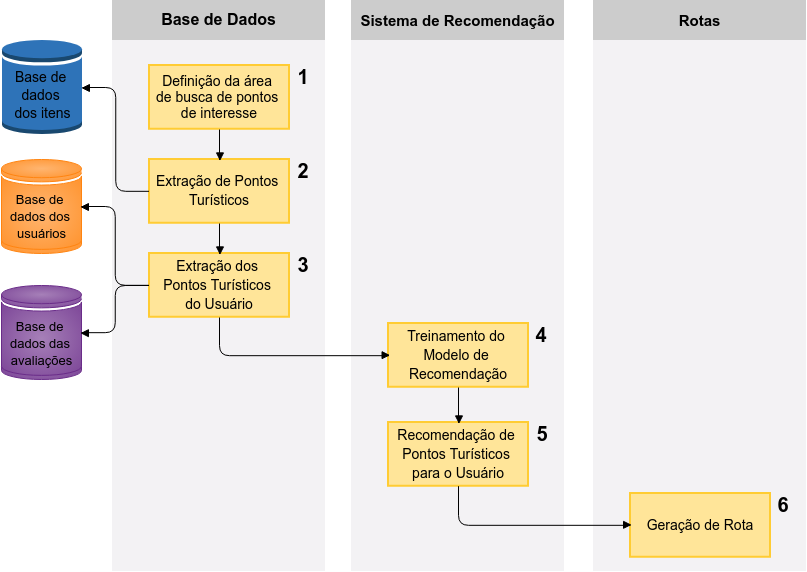
\includegraphics[width=\textwidth]{images/Tourisys_Funcionamento.png}
    \caption{Fluxo do Funcionamento do Sistema.}
    \label{fig:tourisys_operation}
\end{figure}

Diante da base de dados pronta, passa para o passo 4, para o treinamento do modelo do sistema de recomendação. Nessa fase, o sistema está pronto para recomendar pontos turísticos não só para novos usuários mas para também usuários que estão contidos na base de dados formada no passo anterior. No passo 5 é realizada a recomendação de pontos turísticos para o usuário. De acordo com o modelo de recomendação escolhido, o usuário informa pelo menos um local que já tenha visitado e que este esteja contido na base de dados do sistema. Com essas informações, é possível gerar recomendação para aquele determinado usuário com locais que possam ser do interesse do turista.

O último passo é a geração do mapa. É gerada uma página HTML, que mostra a rota que deve ser feita para a visitação dos pontos turísticos, de acordo com o gosto do usuário. Esse mapa é construído através da API do Google Maps, no qual é informado o local de origem e destino e os pontos de parada, que são os pontos do resultado do passo anterior.

\section{Modelo de Usuário}

Para construir o modelo de usuário, é preciso detectar e somar todas as informações básicas do perfil. O modelo de usuário deste projeto segue a metodologia de \cite{Brusilovsky:2001:AH:598284.598341}, incorporando as atividades do usuário. 

Neste trabalho, a princípio, é analisado uma única informação monitorada, favorável para a utilização, que são os conjuntos dos pontos turísticos já visitados pelo usuário. Este conjunto é um forte indicador do interesse do usuário, pois apresenta qual a vontade do turista através da categoria dos locais. Desse modo, este projeto se assemelha muitos com sistemas de recomendação baseados na experiência do usuário, como é apresentado na seção \ref{subsec:eTourism_recsys_userXP}.

A localização de origem e destino do usuário é uma grande utilidade na recomendação de pontos turísticos. Através dessas informações, pode-se sugerir locais turísticos próximos desses pontos. Por enquanto, é necessário o usuário inserir manualmente os pontos de início e fim da rota. Nos trabalhos futuros, essa recomendação poderá ser feita em tempo real, monitorando a localização atual do usuário e sugerindo não só os pontos de interesse, mas também pontos finais da rota. Além disso, pode-se considerar outros pontos turísticos que o usuário visitou através do histórico de localização.

\section{Modelo de Pontos de Interesse}

No nosso contexto, são utilizados para testes dois tipos de modelos de itens, ou pontos de interesse: o modelo baseado em similaridade, através do algoritmo \textit{Item Similarity}; e o modelo baseado em conteúdo, com o algoritmo \textit{Item Content}. Cada modelo trabalha de formas diferentes.

\subsection{Modelo de Pontos de Interesse Baseado em Similaridade}

No modelo de pontos de interesse baseado em similaridade, é necessário calcular a similaridade entre os itens usando as observações dos usuários que interagiram com dois ou mais itens. Dado uma similaridade entre os itens $i$ e $j$, $S(i,j)$ classifica um item $j$ para o usuário $u$ usando uma média ponderada das observações anteriores do usuário $I_u$ \citep{Ricci:2010:RSH:1941884}. Para este modelo utiliza-se o algoritmo \textit{Item Similarity}, que usa as semelhanças de item por item baseado nos usuários em comum para criar a recomendação. Existem diversas métricas de similaridade: \textit{Jaccard}, \textit{Cosine} e \textit{Pearson Correlation}.

\subsubsection{Métricas de Similaridade}
\label{subsubsec:similarity_metrics}

A similaridade \textit{Jaccard} é utilizada para medir a similaridade entre dois conjuntos de elementos \citep{Ricci:2010:RSH:1941884}. No contexto de recomendação, a similaridade \textit{Jaccard} entre dois itens é calculada da seguinte forma:

\begin{equation}
    \mbox{JS}(i,j) = \frac{|U_i \cap U_j|}{|U_i \cup U_j|}
\end{equation}

no qual $U_i$ é o conjuntos de usuários que avaliaram o item $i$. Jaccard é uma boa escolha quando somente contém avaliações implícitas dos itens (exemplo: pessoas avaliaram ou não) ou quando a informação de quantas estrelas o item recebeu não é significativo. Se é necessário a comparação entre as avaliações dos itens, as similaridades \textit{Cosine} e \textit{Pearson Correlation} são recomendadas \citep{Ricci:2010:RSH:1941884}.

A similaridade \textit{Cosine} entre dois itens é calculada da seguinte forma:

\begin{equation}
    \mbox{CS}(i,j) = \frac{\sum_{u\in U_{ij}} r_{ui}r_{uj}}
    {\sqrt{\sum_{u\in U_{i}} r_{ui}^2} \sqrt{\sum_{u\in U_{j}} r_{uj}^2}}
\end{equation}

no qual $U_i$ é o conjuntos de usuários que avaliaram o item $i$ e $U_ij$ é o conjunto de usuários que avaliaram tanto o item $i$, tanto o item $j$. Um dos problemas da similaridade \textit{Cosine} é que ela não considera as diferenças entre a média e a variância das avaliações feitas para os itens $i$ e $j$ \citep{Ricci:2010:RSH:1941884}. Para resolver este problema, a similaridade \textit{Pearson Correlation} compara avaliações, removendo os efeitos das médias e das variâncias. Calcula-se esse coeficiente segundo a fórmula:

\begin{equation}
    \mbox{PS}(i,j) = \frac{\sum_{u\in U_{ij}} (r_{ui} - \bar{r}_i)(r_{uj} - \bar{r}_j)}
    {\sqrt{\sum_{u\in U_{ij}} (r_{ui} - \bar{r}_i)^2} \sqrt{\sum_{u\in U_{ij}} (r_{uj} - \bar{r}_j)^2}}
\end{equation}

em que $U_ij$ é o conjunto de usuários que avaliaram os itens $i$ e $j$; $r_ui$ é a avaliação que o usuário $u$ deu ao item $i$; $r_uj$ é a avaliação que o usuário $u$ deu ao item $j$, $\bar{r}_i$ é a media das avaliações do item $i$ e $\bar{r}_j$ é a media das avaliações do item $j$.

\subsection{Modelo de Pontos de Interesse Baseado em Conteúdo}

No modelo de pontos de interesse baseado em conteúdo, o índice de similaridade entre dois itens é calculado pela primeira vez que mede a similaridade entre os dados do item para cada coluna. Em seguida, é medida a média ponderada das similaridades por coluna, para obter a semelhança final. As recomendações são geradas de acordo com a similaridade média de um item candidato com todos os itens no conjunto de itens classificados de um usuário.

Nesse cenário, as informações relevantes que são consideradas são as categorias e a localização. A categoria diz respeito ao que é o ponto turístico, caracterizando-o de acordo com o que o local oferece ao turista. A localização fornece informações específicas de latitude e longitude do local. Todas as duas informações são pré-definidas e não precisam da interação do usuário. Formalmente, o modelo de pontos de interesse baseado em conteúdo é um par $(C,L)$:

\begin{itemize}
    \item $C$ representa o conjunto de categorias do ponto turístico. As categorias são pré-definidas e estáticas enquanto não houver uma atualização no sistema do OpenStreetMap\footnote{https://www.openstreetmap.org/} que as modifique. Cada elemento do conjunto de categorias tem a mesma importância para este modelo.
    \item $L$ representa a localização do ponto turístico. As localizações são pré-definidas e estáticas. Especificamente, a localização é composta da latitude e longitude do local.
\end{itemize}

Outras informações sobre o ponto de interesse em si, como nome, também podem ser úteis. Para melhor entendimento, o seguinte exemplo mostra o modelo de um ponto turístico:

\begin{itemize}
    \item $C = \{"arts\_centre", "attraction"\}$ representam as categorias da loja, indicando que é um local de centro de artes e uma atração;
    \item $L$ = (-12.9995737,-38.5296316), que representa a latitude e longitude do ponto turístico, respectivamente.
\end{itemize}

\section{Sumário}

Neste capítulo, mostra-se uma visão geral sobre os aspectos do desenvolvimento do sistema. Discutiu-se sobre a arquitetura do sistema, abordando os aspectos da estrutura do sistema. Foram apresentadas as ferramentas e tecnologias utilizadas e como é o funcionamento do sistema construído. No próximo capítulo \ref{chp:evaluation} será realizada uma avaliação do trabalho realizado, discutidas metodologia, métricas de avaliação e os resultados obtidos.
\chapter{Avaliação}
\label{chp:evaluation}

Neste capítulo, será mostrado o processo de avaliação utilizado para verificar se os objetivos previstos foram alcançados. Espera-se que com a criação de rotas de pontos turísticos o usuário possa visitar a maior quantidade de lugares dentro da sua rota de origem e destino. Para isso, os experimentos aqui utilizam o OpenStreetMap e Google Maps como fonte de dados, tanto de usuário, tanto dos domínios de pontos de interesses. A avaliação consiste em comparar as combinações de diferentes tipos de metadados, utilizando os algoritmos de sistemas de recomendações. Também serão apresentados neste capítulo os detalhes da metodologia utilizada para desenvolver e avaliar este trabalho, bem como o conjunto de dados utilizados durante os experimentos. Em seguida, são apresentadas as métricas utilizadas na avaliação e os resultados obtidos. Por fim, é feita uma discussão e apresentados pontos de melhoria.

\section{Metodologia}

Os testes realizados para a avaliação tem por objetivo mostrar que é possível recomendar pontos turísticos de acordo com as preferências do usuário. Além disso, os testes exibem a precisão das recomendações, de acordo com as atribuições escolhidas para análise e o modelo de recomendação.

Para avaliar os modelos serão realizadas comparações, variando de acordo com os dados que cada um dos modelos utilizam para gerar as recomendações. No caso do modelo \textit{Item Similarity}, diferenciou-se o tipo de similaridade entre \textit{Jaccard}, \textit{Cosine} e \textit{Pearson Correlation}, mencionados em \ref{subsubsec:similarity_metrics}. Já no caso do \textit{Item Content}, intercalou-se entre os atributos da base de dados de itens. Considerando as informações do ID do item, as combinações foram: somente uma categoria; uma ou mais categorias; somente localização; localização e uma categoria; localização e uma ou mais categorias; nome; nome e somente uma categoria; nome e uma ou mais categorias; nome e localização; nome, somente uma categoria e localização; e todas as atribuições. 

Para os testes, utilizou-se o processo de \textit{Cross-Validation}, criando conjuntos de treino e de teste. Utilizando o conjunto de treino, o modelo é treinado e testa-se com os exemplos do conjunto de teste. Depois, diferentes conjuntos de treino e de teste são selecionados para iniciar o processo de treino e teste novamente, sendo repetido $k$ vezes \citep{Ricci:2010:RSH:1941884}. Com os arquivos e os modelos mencionados anteriormente, todos os testes foram realizados com a biblioteca GraphLab\footnote{https://turi.com/}. Para medir a precisão de cada uma das comparações, foram utilizadas as métricas \ac{rmse}, \textit{Precision}, \textit{Recall} e F-\textit{Score}.


\section{Conjunto de Dados}

Os testes foram executados com dados oriundos de diversas fontes. Primeiramente, foram coletados dados do OpenStreetMap\footnote{https://www.openstreetmap.org} para obter informações sobre pontos de interesse relacionados a turismo da cidade de Salvador e quais são suas categorias. Depois, foram coletados dados do Google Maps para obter \textit{reviews} dos locais. Devido a limitação da API do Google, a ferramenta só disponibiliza as 5 últimas avaliações de cada ponto de interesse. Portanto, cada local tem, no máximo, 5 \textit{ratings}. Além disso, alguns locais tem mais de uma categoria. No total, o banco de dados foi composto de 178 usuários, 52 pontos de interesse de 12 tipos diferentes e 227 avaliações, como pode ser visto na Tabela \ref{tab:dataset_Salvador}

\begin{table}[H]
	\centering
	\caption{Conjunto de Dados de POI da cidade de Salvador.}
	\label{tab:dataset_Salvador}
	\begin{tabular}{|c|c|}
		\hline
		\multicolumn{2}{|c|}{\textbf{Conjunto de Dados}} \\ \hline
		Usuários                  & 178                   \\ \hline
		Pontos de Interesses      & 52                   \\ \hline
		Categorias de POI         & 12                 \\ \hline
		Avaliações                & 227                 \\ \hline
	\end{tabular}
\end{table}


Existem várias técnicas de \textit{Cross-Validation}, aqui foi utilizada a técnica através da porcentagem dos dados que devem ser mantidos para treino e para teste, devido a pouca quantidade de avaliações no conjunto de dados. Neste projeto, a proporção que foi de 80\% para o conjunto de treino e 20\% para o conjunto de testes para criar o conjunto de validação. Os algoritmos utilizados foram os de \textit{Item Similarity}, ou Similaridade de Itens e \textit{Item Content}, em português Conteúdo dos Itens.

\section{Métricas de Avaliação}

Em um sistema de recomendações, é fornecido ao usuário uma lista de recomendações. ele pode avaliar os itens como relevantes ou não relevantes. Essas métricas são conhecidas como Precisão (\textit{Precision}, em inglês) e \textit{Recall}. São utilizadas na recuperação de informação e úteis para avaliar a qualidade de um modelo de recomendação \citep{ParraSahebi2013}. Precisão é a fração dos itens recomendados que são relevantes \citep{Manning:2008:IIR:1394399}, sendo definida como

\begin{equation}
    precision = \frac{itens~relevantes~recomendados}{itens~na~lista}~~,
\end{equation}

Recall é definida como a fração de recomendações relevantes que são apresentadas para o usuário:

\begin{equation}
    recall = \frac{itens~relevantes~recomendados}{itens~relevantes}~~,
\end{equation}

\subsection{Precisão em n (\textit{P@n})}

As métricas de avaliação irão considerar apenas os itens do topo, chamados de Top-N recomendações, e são normalmente apresentados como precisão em n (\textit{P@n}). Isso acontece pois o número de itens recomendados em uma lista pode ser muito alto, dependendo do modelo de recomendação e do tamanho do conjunto de dados. \textit{P@n} é utilizado para avaliar o sistema no contexto de um único usuário. A equação de \textit{P@n} que mede a relevância dos $n$ primeiros itens da uma lista é:

\begin{equation}
    P@n = \frac{r}{n}~~,
\end{equation}

no qual $n$ é o número de itens retornados e $r$ é o número de itens considerados relevantes e retornados até a posição $n$ da lista.

\subsection{Recall em n (\textit{R@n})}

Assim como a precisão, Recall também considera apenas os itens do topo, os Top-N recomendações. A equação de \textit{R@n} que mede a proporção de itens relevantes que foram recomendados de entre todos os relevantes é:

\begin{equation}
    R@n = \frac{e}{n}~~,
\end{equation}

no qual5.3ondené $n$ é o número de itens relevantes e recomendados e $e$ é o número de itens relevantes até a posição $n$ da lista.

Tanto o resultado do \textit{Precision}, tanto o resultado do \textit{Recall} variam entre 0 e 1. Quanto mais alto for o valor, melhor é a performance do modelo. Se o valor da \textit{Precision} for 1, significa que todos os itens recomendados são relevantes, no entanto, não se sabe se todos os relevantes foram recomendados. Caso o valor do \textit{Recall} seja 1, mostra que todos os itens relevantes foram recomendados, mas não se sabe quantas recomendações não são relevantes \citep{morais2012sistemas}.

Essas duas medidas são inversamente relacionadas e sozinhas não permitem avaliar completamente o sistema. Aumentando o número de itens recomendados, o \textit{Recall} tem tendencia a aumentar porque maior é a probabilidade de os itens relevantes serem selecionados, assim como a \textit{Precision} diminui. Por isso, escolheu-se uma outra medida que incremente na análise da avaliação \citep{morais2012sistemas}.

\subsection{F1-\textit{Score}}

F1-\textit{Score} é a média ponderada de \textit{Precision} e \textit{Recall}, ou seja, é o equlibrio entre a precisão e o recall. Essa medida é definida pela seguinte expressão:

\begin{equation}
    F_1 = 2 \cdot \frac{precision \cdot recall}{precision + recall}.
\end{equation}

Assim como a \textit{precision} e o \textit{recall}, F1 varia igualmente entre 0 e 1. Quanto maior for o valor, melhor é o resultado da avaliação. Como neste trabalho está sendo utilizado dois modelos de recomendação e verificando os seus resultados, está medida vai ser utilizada principalmente para a avaliação de performance do algoritmo de recomendação.

\subsection{\textit{Root Mean Square Error (RMSE)}}

Para mensurar como está a acurácia do sistema de recomendação, é preciso utilizar além da precisão e da cobertura, que classificam os itens como boas ou más recomendações, é possível utilizar de métricas para averiguar a classificação dos itens em uma determinada escala \citep{Jannach:2010:RSI:1941904}. Nesse projeto, foi utilizado o \textit{RMSE}. Basicamente, o \textit{RMSE} calcula o desvio entre as avaliações previstas e as reais avaliações porém coloca mais ênfase no maior desvio \citep{Jannach:2010:RSI:1941904}. A equação de \textit{RMSE} é:

\begin{equation}
    RMSE = \sqrt{\frac{1}{N} \sum_{i=1}^{N} (p_i - r_i)^2}
\end{equation}

, supondo que $p$ e $r$ são vetores de tamanho $N$ e que $r$ contém as reais avaliações e $p$ as avaliações previstas. O valor do \ac{rmse} é o mesmo do atributo escolhido para ser a variável dependente. Tanto no \textit{Item Content}, tanto no \textit{Item Similarity}, a variável escolhida é o valor da nota atribuído ao item pelos usuários, que varia entre 1 a 5.

\section{Resultados}

Para avaliar os resultados foram utilizadas as seguintes métricas de avaliação:

\renewcommand{\labelenumi}{\roman{enumi})}
\begin{enumerate}
    \item \acfi{rmse}, o desvio entre as avaliações previstas e as reais;
    \item Precisão, que calcula o percentual de itens recomendados que são relevantes;
    \item Recall, que calcula o percentual de itens relevantes que foram recomendados;
    \item F1-\textit{Score}, a média ponderada entre precisão e recall.
\end{enumerate}

Os valores de cada métrica estão na Tabela \ref{tab:results_item_similarity}, que mostra os resultados para o modelo de recomendação \textit{Item Similarity} de acordo com os tipos de similaridade; a Tabela \ref{tab:results_item_content}, que apresenta os resultados para o modelo \textit{Iem Content}, de acordo com os atributos de itens que foram utilizados em cada teste. A Tabela \ref{tab:all_results} mostra os resultados dos dois modelos. Na identificação, foram utilizadas as seguintes convenções: [IS-XX] para os testes com \textit{Item Similarity} e [IC-XX] para os testes com \textit{Item Content}, no qual os números são de acordo com a coluna \textit{ID} das Tabelas \ref{tab:results_item_similarity} e \ref{tab:results_item_content}.

\begin{table}[H]
    \centering
    \caption{Resultados para \textit{RMSE}, \textit{P@10} e \textit{R@10} no modelo \textit{Item Similarity}.}
    \label{tab:results_item_similarity}
    \begin{tabular}{|c|c|c|c|c|c|}
        \hline
        \textit{ID} & 
        \textit{Tipo de Similaridade} & 
        \textit{RMSE} & 
        \textit{P@10} & \textit{R@10} & F1-\textit{Score} \\ \hline
        01 & Jaccard & 4.42010 & 0.01250 & 0.11250 & 0.02250 \\ \hline
        02 & Cosine & 4.35065 & 0.01250 & 0.11250 & 0.02250 \\ \hline
        03 & Pearson Correlation & \textbf{1.37313} & \textbf{0.03000} & \textbf{0.25000} & \textbf{0.05357} \\ \hline
    \end{tabular}
\end{table}

\subsection{\acfi{rmse}}

A métrica \acl{rmse} foi utilizada para medir o desvio de erro do algoritmo. Analisando os resultados obtidos pelo \ac{rmse} nas tabelas, conclui-se que existe um desvio muito grande entre as avaliações previstas e as reais.

No nosso projeto, essa métrica é avaliada da seguinte forma: no caso do modelo \textit{Item Similarity}, é esperado que o sistema de recomendação sugira pontos turísticos semelhantes ao que o usuário já avaliou, com base em usuários em comum. Ou seja, se um usuário visitou o Museu Náutico da Bahia, a preferência é que sejam recomendados pontos turísticos semelhantes com outros itens da base de dados para o usuário em questão. Já no modelo \textit{Item Content}, a semelhança entre os itens recomendados é determinado pelo conteúdo desses itens, ao invés de usar padrões de interação do usuário para calcular a similaridade. Voltando ao exemplo do Museu Náutico da Bahia, que se encaixa na categoria museu, este modelo irá recomendar pontos turísticos com a mesma categoria, no caso, irá sugerir outros museus.

No modelo \textit{Item Similarity}, o que menos teve erros foi o modelo \textit{Pearson}, com o valor de 1.37313 e o maior foi o do Jaccard, com 4.42010. Já no \textit{Item Content}, o menor (mas não o melhor), foi quando utilizou o atributo Localização e o pior foi o com a característica Nome. Este resultado era de se esperar, pois a base de dados ainda está muito incipiente: existe poucos usuários com mais de uma avaliação em diferentes itens, o que compromete com os resultados obtidos. Quanto mais usuários com mais e mais avaliações, melhor será a predição e a recomendação para futuros usuários.

\subsection{P@10 e R@10}

O P@10 considera a precisão dos dez primeiros itens da lista, pontuando mais os acertos nos dez primeiros itens. Analisando os resultados, no modelo \textit{Item Similarity}, este valor foi igual tanto no \textit{Jaccard} tanto no \textit{Cosine}. O melhor valor foi obtido pelo tipo de similaridade \textit{Pearson Correlation}. No caso de \textit{R@10}, o melhor resultado foi obtido também no tipo de similaridade \textit{Pearson Correlation}, ligeiramente maior comparado a \textit{Cosine} e \textit{Jaccard}, estes que tiveram o mesmo valor.

\begin{table}[H]
    \centering
    \caption{Resultados para RMSE, P@10 e R@10 no modelo \textit{Item Content}.}
    \label{tab:results_item_content}
    \begin{tabular}{|c|p{15em}|c|c|c|c|}
        \hline
        \multicolumn{1}{|>{\centering}c|}{\textit{\textbf{ID}}} &
        \multicolumn{1}{>{\centering}p{15em}|}{\textit{\textbf{Atributos de Itens}}} &
        \multicolumn{1}{>{\centering}c|}{\textit{\textbf{RMSE}}} &
        \multicolumn{1}{>{\centering}c|}{\textit{\textbf{P@10}}} &
        \multicolumn{1}{>{\centering}c|}{\textit{\textbf{R@10}}} &
        \multicolumn{1}{>{\centering}c|}{\textit{\textbf{F1-\textit{Score}}}} \\ \hline
        01 & Somente uma categoria & 4.06223 & 0.02750 & 0.23750 & 0.04929 \\ \hline
        02 & Uma ou mais categorias & 4.09162 & 0.03500 & 0.30000 & 0.06269 \\ \hline
        03 & Localização & \textbf{3.41135} & 0.04000 & 0.31875 & 0.07108 \\ \hline
        04 & Localização e somente uma categoria & 3.50065 & 0.05000 & 0.43750 & 0.08974 \\ \hline
        05 & Localização e uma ou mais categorias & 3.56493 & \textbf{0.05250} & \textbf{0.47500} & \textbf{0.09455} \\ \hline
        06 & Nome & 4.39682 & 0.03000 & 0.26875 & 0.05397 \\ \hline
        07 & Nome e somente uma categoria & 4.18395 & 0.04250 & 0.37500 & 0.07635 \\ \hline
        08 & Nome e uma ou mais categorias & 4.21318 & 0.04750 & 0.42500 & 0.08545 \\ \hline
        09 & Nome e localização & 3.64087 & 0.04250 & 0.33125 & 0.07533 \\ \hline
        10 & Nome, localização e somente uma categoria & 3.64233 & 0.04750 & 0.41250 & 0.08519 \\ \hline
        11 & Todos os atributos & 3.72535 & \textbf{0.05250} & \textbf{0.47500} & \textbf{0.09455} \\ \hline
    \end{tabular}
\end{table}

No \textit{Item Content}, o \textit{Precision} e o \textit{Recall} tiveram uma melhora de aproximadamente 75\% e 90\% respectivamente, comparado entre o maior valor do \textit{Item Similarity} e do \textit{Item Content}. O maior valor alcançado pelo \textit{P@10} foi obtido ao utilizar os atributos de localização e uma ou mais categorias do item, obtendo um valor de 0.05250. Neste caso, o valor de \textit{R@10} também foi o melhor, tendo uma grandeza de 0.47500. Como o atributo localização define a latitude e a longitude do ponto turístico, deduz-se que com essa análise que quanto mais próximo um item do outro, mais relevante será este item no momento de recomendar ao usuário. Adicionando a atribuição de uma ou mais categorias, considera-se que as recomendações são de itens com categorias semelhantes e próximas entre si.

O menor valor alcançado pelo \textit{P@10} no \textit{Item Content} foi quando foi utilizado o atributo Somente uma categoria. O mesmo aconteceu no caso do \textit{R@10}. Compreende-se que este resultado se deu devido ao fato que quando utilizado somente uma categoria, os itens que tem mais de um são repetidos na base com categorias diferentes. Ou seja, são itens iguais mais como as categorias são diferentes, a semelhança entre eles não são totalmente idênticos.

\subsection{F1-\textit{Score}}

Como foi explicado anteriormente, F1-\textit{Score} nos dá uma média ponderada entre o \textit{Precision} e o \textit{Recall}. Analisando a sua equação, conclui-se que quanto maior o valor do \textit{Precision} e do \textit{Recall}, maior será o valor do F1-\textit{Score}. Logo, seguindo essa linha de raciocínio, verifica-se que os melhores F1-\textit{Score} são com o tipo de similaridade \textit{Pearson Correlation} em \textit{Item Similarity} e na escolha dos atributos Localização e uma ou mais categorias e quando utiliza todas as características do item em \textit{Item Content}. Deduz que, considerando essa métrica para escolher o melhor algoritmo de acordo com sua performance, o algoritmo escolhido seria \textit{Item Content}.

\begin{table}[H]
    \centering
    \caption{Resultados para RMSE, P@10 e R@10 em todos os modelos.}
    \label{tab:all_results}
    \begin{tabular}{|c|c|c|c|c|}
        \hline
        \textit{Modelo e número} &
        \textit{RMSE} & 
        \textit{P@10} & \textit{R@10} & F1-\textit{Score}\\ \hline
        IS-01 & 4.42010 & 0.01250 & 0.11250 & 0.02250 \\ \hline
        IS-02 & 4.35065 & 0.01250 & 0.11250 & 0.02250 \\ \hline
        IS-03 & \textbf{1.37313} & 0.03000 & 0.25000 & 0.05357 \\ \hline
        IC-01 & 4.06223 & 0.02750 & 0.23750 & 0.04929 \\ \hline
        IC-02 & 4.09162 & 0.03500 & 0.30000 & 0.06269 \\ \hline
        IC-03 & 3.41135 & 0.04000 & 0.31875 & 0.07108 \\ \hline
        IC-04 & 3.50065 & 0.05000 & 0.43750 & 0.08974 \\ \hline
        IC-05 & 3.56493 & \textbf{0.05250} & \textbf{0.47500} & \textbf{0.09455} \\ \hline
        IC-06 & 4.39682 & 0.03000 & 0.26875 & 0.05397 \\ \hline
        IC-07 & 4.18395 & 0.04250 & 0.37500 & 0.07635 \\ \hline
        IC-08 & 4.21318 & 0.04750 & 0.42500 & 0.08545 \\ \hline
        IC-09 & 3.64087 & 0.04250 & 0.33125 & 0.07533 \\ \hline
        IC-10 & 3.64233 & 0.04750 & 0.41250 & 0.08519 \\ \hline
        IC-11 & 3.72535 & \textbf{0.05250} & \textbf{0.47500} & \textbf{0.09455} \\ \hline
    \end{tabular}
\end{table}

\subsection{Análise Geral}

No geral, analisando todos os modelos e suas variações, conclui-se que o melhor modelo que possível de utilizar, considerando a atual base de dados, é o de \textit{Item Similarity} com o tipo de similaridade \textit{Pearson Correlation}. Apesar deste modelo não ter tido bons números na \textit{Precision} e no \textit{Recall}, consequentemente no F1-\textit{Score}, o desvio de erro entre as avaliações previstas e as reais avaliações foi o menor de todos e um valor que pode ser considerado em futuras avaliações.

Além disso, nessa pesquisa conclui-se que o fato de que os modelos com maiores valores de \textit{Precision} e \textit{Recall} tiveram valores de \ac{rmse} muitos altos. Ou seja, antes de escolher um modelo de recomendação através do índice que mede sua performance, é necessário observar outras métricas para avaliar se o algoritmo é o ideal de acordo com seus objetivos e sua base de dados.

\subsection{Rotas}

Após o treino do sistema de recomendação dos pontos de interesse, é possível recomendar pontos turísticos a um determinado usuário, de acordo com as suas preferências, e assim gerar a rota. Para exemplificar as rotas, considere um usuário que já visitou o Elevador Lacerda e avaliou com a nota 4.0. No momento, ele se encontra no Terminal Marítimo de Passageiros do Porto de Salvador e tem como destino o Largo Terreiro de Jesus. Utilizando esses dados e, de acordo com a análise anterior, utilizando os modelos \textit{Item Similarity} com o tipo de similaridade \textit{Pearson Correlation}; e \textit{Item Content} com todos os atributos, seguem os resultados dos pontos recomendados e das rotas. As Figuras \ref{fig:IS_pearson_newUser_results_rotate} e \ref{fig:IS_pearson_newUser_route} são, respectivamente, os pontos de interesse sugeridos e a rota do modelo \textit{Item Similarity}. Já as Figuras \ref{fig:IC-loc_item-newUser-results_rotate} e \ref{fig:IC-loc_item-newUser-route} são, respectivamente, os pontos de interesse sugeridos e a rota do modelo \textit{Item Content}.

\begin{sidewaysfigure}
    \centering
    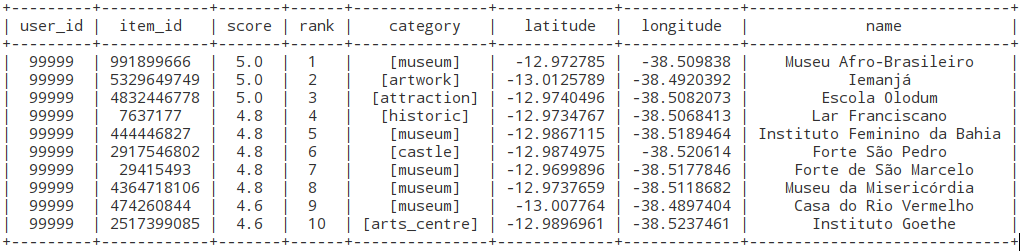
\includegraphics[scale=0.95]{images/IS_pearson_newUser_results.png}
    \caption{Exemplo de um resultado do sistema de recomendação para o novo usuário pelo modelo \textit{Item Similarity}.}
    \label{fig:IS_pearson_newUser_results_rotate}
\end{sidewaysfigure}

\begin{sidewaysfigure}
    \centering
    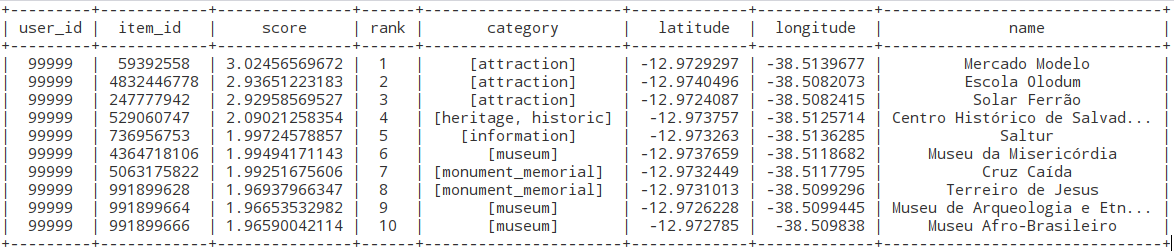
\includegraphics[scale=0.85]{images/IC-loc_item-newUser-results.png}
    \caption{Exemplo de um resultado do sistema de recomendação para o novo usuário pelo modelo \textit{Item Content}.}
    \label{fig:IC-loc_item-newUser-results_rotate}
\end{sidewaysfigure}

\begin{figure}
    \centering
    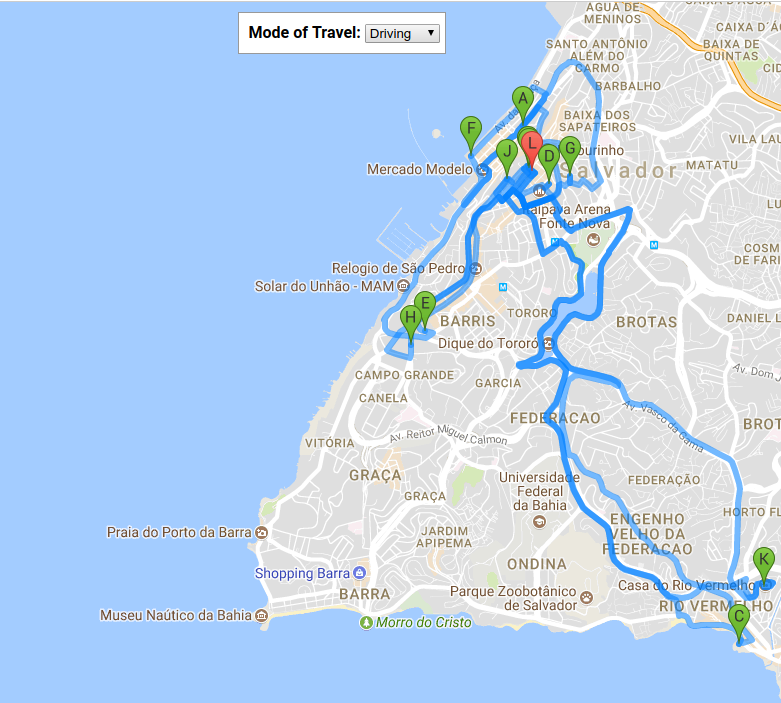
\includegraphics[scale=0.6]{images/IS_pearson-newUser-route.png}
    \caption{Exemplo de um resultado da rota para o novo usuário pelo modelo \textit{Item Similarity}.}
    \label{fig:IS_pearson_newUser_route}
\end{figure}

\begin{figure}
    \centering
    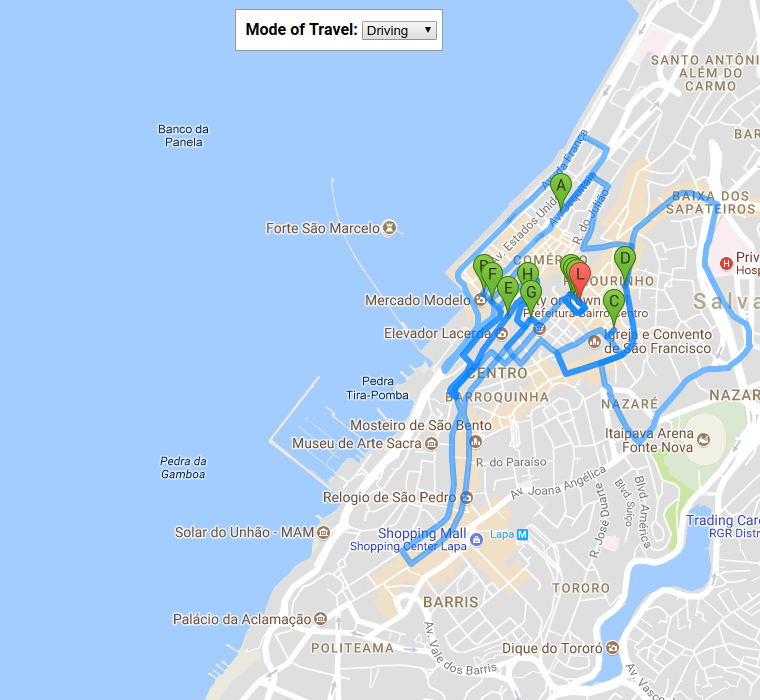
\includegraphics[scale=0.6]{images/IC-loc_item-newUser-route.png}
    \caption{Exemplo de um resultado da rota para o novo usuário pelo modelo \textit{Item Content}.}
    \label{fig:IC-loc_item-newUser-route}
\end{figure}


\section{Discussão}

Neste trabalho foi mostrado a construção de um sistema de recomendação de rotas de pontos turísticos com base em filtragem colaborativa. Em meio a tantas informações, este sistema de recomendação pode ajudar o turista que deseja conhecer pontos turísticos da cidade que está visitando mas não sabe quais pontos ir e que rota seguir.

Após analisar os resultados obtidos com as métricas utilizadas,  conclui-se que é possível fazer recomendações de acordo com as preferências do usuário e gerar rotas considerando sua origem e destino. Ainda não chega a ser um resultado bom, devido a diversos fatores, mas é algo a ponderar, analisando de que forma será possível melhorar para encontrar um modelo de recomendação que seja o ideal para este tipo de recomendação.

Além disso, este trabalho serve como um começo para serviços relacionados a área de turismo possam implementar sistemas de recomendação para os seus usuários, gerando rotas que facilitem a excursão do turista durante a sua viagem. O Apontador \footnote{https://www.apontador.com.br/}, site de busca de lugares, serviços e facilidades, pode fazer uso da abordagem proposta neste trabalho para fazer sugestão de pontos de acordo com as avaliações feitas pelos usuários que o site já tem cadastrado, além de gerar rotas de acordo com as suas preferências.

\section{Pontos de Melhoria}

Durante a realização deste projeto, houveram alguns problemas que podem ter impactado no resultado deste trabalho. Um dos principais problemas foi na obtenção de dados através da API do Google Maps. Como foi citado no capítulo 4 sobre o funcionamento do sistema \ref{sec:operation}, para fazer a busca do local no Google Places, era necessário informar o nome e a localização do ponto de interesse, o que trouxe problemas relacionados a error de grafia ou ruídos, como em casos em que naquela localização não havia um local com aquele nome, trazendo um outro local próximo. Muitos casos foram resolvidos, mais ainda é um ponto a se considerar como melhoria.

Outro problema é a limitação da quantidade de avaliações por local da API do Google Maps, impactando na quantidade de itens por usuário no banco de dados. Por conta disso, item que contém mais de 1000 avaliações, somente são considerados as cinco últimas análises. Além disso, não é disponibilizado muitas informações de usuários, impossibilitando trabalhar com modelos de recomendação voltados ao usuário.

Algo a acrescentar que pode ajudar nos futuros trabalhos é a ampliação do banco de dados para outras áreas além da cidade de Salvador. Para a realização de testes, foi utilizada somente pontos turísticos de Salvador, criando um impasse para turistas que nunca vieram a Salvador, mas já foram em outros pontos turísticos de outras regiões do Brasil mas que não etão na base de dados.

Para finalizar, o modelo \textit{Item Content} é um algoritmo recentemente implementado na ferramenta GraphLab, atualmente sendo um algoritmo no estado beta. Por conta disso, talvez alguns resultados possam ter sido prejudicado por conta de erros ou \textit{bugs} que o algoritmo possa a ter. Com tudo isso, existe ainda muitos pontos a serem melhorados e explorados, gerando novos dados, seguindo a proposta apresentada neste trabalho.

\section{Sumário}

Este capítulo apresentou os principais resultados obtidos durante o desenvolvimento dos experimentos para avaliar a implementação de um sistema de recomendação de rotas de pontos turísticos. No começo, foram apresentadas as metodologias de avaliação utilizadas no estudo, a base de dados a as métricas utilizadas. O estudo apresentado neste capítulo mostrou que é possível construir um sistema de recomendação que auxilie os turistas nas suas próximas viagens, conhecendo novos lugares de acordo com os seus interesses.
\chapter{Conclusão}
\label{chp:conclusion}

Neste trabalho foi apresentado um sistema de recomendação de rotas de pontos turísticos. Inicialmente foi apresentado a motivação para a criação do sistema de recomendação, relatou-se alguns problemas que os turistas enfrentam para montar seu itinerários para as próximas viagens. Foi proposta uma solução para ajudar os usuários a encontrar pontos turísticos de sua preferência, usando um sistema de recomendação que gera uma rota para esses pontos.

No Capítulo \ref{chp:recSys} descreve sobre os sistemas de recomendação,  apresentando um histórico, discussão de conceitos quanto aos dados que são utilizados em um sistema além das tarefas desempenhadas pelos sistemas de recomendação e as suas principais técnicas.

No Capítulo \ref{chp:eTourism} apresentou-se sobre o setor turístico, mostrando os principais conceitos e descrevendo trabalhos relacionados a sistemas de recomendações com foco no turismo. Exemplificou sistemas que disponibilizam informações relacionadas ao turismo além de de como são classificadas os sistemas de recomendação para \textit{e-Tourism}.

O Capítulo \ref{chp:eTourismRecSys} explica a proposta de solução para a recomendação de rotas de pontos turísticos para o turista. Foi apresentado os requisitos funcionais e não funcionais do software desenvolvido, a sua arquitetura e as tecnologias utilizadas. Esclarece todo o seu funcionamento para o usuário além de expor sobre os modelos do usuário e do item.

Para finalizar, o sistema de recomendação foi apresentado em detalhes e realizou-se uma avaliação experimental. Os métodos de avaliação e os resultados foram apresentados, mostrando o êxito da proposta, ou seja, a recomendação de pontos turísticos de acordo com as preferências do turista e a geração da rota de acordo com o resultado. A seguir, menciona as contribuições principais deste trabalho e os trabalhos futuros.

\section{Contribuição do Trabalho}

As principais contribuições deste trabalho são explicados a seguir:

\begin{itemize}
    \item \textbf{Revisão de sistemas de recomendação voltadas ao turismo:} Neste projeto, desempenhou-se uma revisão de sistemas de recomendação focados na área do turismo, mostrando-se os trabalhos relacionados. Além disso, o estudo proporciona conhecer funcionalidades e diferentes tipos de sistemas de recomendação que poderiam ser utilizados em diferentes cenários para sugestão de pontos turísticos e construção de rotas.
    
    \item \textbf{Modelos de pontos de interesse:} Para testes, foram utilizados dois modelos de recomendação em cima dos itens disponíveis para o nosso sistema. No primeiro, mostra-se como as avaliações de outros usuários podem ajudar na recomendações de outros pontos turísticos. No segundo, classifica-se algumas informações úteis para as recomendações,. Todas as duas, focadas em uma recomendação de acordo com as preferências do turista.
    
    \item \textbf{Avaliações do Experimento:} Com o sistema de recomendação pronto, foram feitos testes para avaliar os dois modelos de recomendação. Foram realizados diversos testes, diferenciando os métodos de similaridade e os atributos do banco de dados dos itens. Fazendo uma comparação, é possível definir as condições de utilizar os modelos de recomendação e suas limitações.
\end{itemize}

\section{Trabalhos Futuros}

Mesmo com os resultados, é possível melhorar ainda mais o sistema de recomendação e a geração de rotas das seguintes formas:

\begin{itemize}
    \item \textbf{Aumento na base de dados de itens e avaliações:} Verificou-se que a limitação de avaliações por itens impactou fortemente nos resultados. Enriquecer essa base, aumentando a quantidade de avaliações por locais e colocar outros pontos turísticos além da cidade de Salvador melhorará a recomendação para os dois modelos apresentados.
    
    \item \textbf{Inserir mais atributos para o usuário:} Acrescentando mais características do usuário, será possível refinar mais as recomendações. Será possível verificar quais são os tipos de pontos turísticos são mais visitados de acordo com o gênero, o país de origem ou a idade do turista.
    
    \item \textbf{Localização do usuário no modelo de recomendação:} Atualmente os dados relacionados a latitude e longitude do usuário são obtidos manualmente para a geração de rotas. Obter essa informação automaticamente é um passo para utilizar a localização na recomendação dos pontos turísticos mais próximos do usuário.
    
    \item \textbf{Melhoria das rotas:} Oferecer ao usuário a menor rota entre os pontos turísticos recomendados, ou tornar o ponto final da rota opcional, sugerindo outros pontos como o último destino do itinerário são passos para aperfeiçoar na geração de rotas para o turista. Além disso, ser possível definir a quantidade de pontos na rota a partir de um algoritmo para definir a quantidade baseada no comprimento da rota, duração, entre outros fatores.
    
    \item \textbf{Criar uma ontologia com base nas avaliações:} Durante essa pesquisa, verificou-se a limitação das APIs dos sistemas de informação quanto a obtenção de avaliações do usuário sobre determinado ponto. Além disso, cada um utiliza um vocabulário diferente na inserção de metadados nas páginas Web. A criação de uma ontologia capaz de agrupar todos esses dados é uma maneira de unificar todas as informações disponíveis em diferentes sistemas de informações.
\end{itemize}

\section{Sumário}

Este capítulo apresentou um resumo de tudo que foi feito e discutido neste projeto. Mostrou-se as principais contribuições da nossa proposta de sistema de recomendação, os objetivos alcançados e os pontos de melhorias do nosso sistema de recomendação para os trabalhos futuros.

% References

\begin{references}
  \bibliography{references}
\end{references}

\end{document}
